\documentclass{beamer}

\usepackage{beamerthemeCambridgeUS}
\usepackage{graphics}
\usepackage{graphicx}
\usepackage{hyperref}
\usepackage{StyleFiles/algorithm}
\usepackage{StyleFiles/algorithmic}
\usepackage{amssymb}
\usepackage{fancyhdr}
\usepackage{eucal}
\usepackage[T1]{fontenc}
\usepackage{lmodern}
\usepackage{amsthm}
\usepackage{pgf}
\usepackage{tikz}
\usetikzlibrary{positioning}
\usetikzlibrary{arrows,automata}
\usepackage{tabularx}
\usepackage{booktabs}
\usepackage{amsmath}
\usepackage{multirow}
\usepackage{layouts}
\usepackage{array}
\usepackage[english,greek]{babel}
\usepackage[iso-8859-7]{inputenc}

\title[Player Behavior and Team Strategy]{Player Behavior and Team Strategy in Robocup Simulation 3D League}
\author[Georgios Methenitis]{Georgios Methenitis}
\institute[TUC]{Technical University of Crete}
\date[Chania, 2012]{Chania, August, 2012}
\subject{Computational Sciences}

\begin{document}


\selectlanguage{english}
\newcommand{\putat}[3]{\begin{picture}(0,0)(0,0)\put(#1,#2){#3}\end{picture}}

  \frame
  {
    \titlepage
    \begin{center}
    \begin{small}
     Thesis Committee\\
    Assistant Professor Michail G. Lagoudakis (ECE)\\
Assistant Professor Georgios Chalkiadakis (ECE)\\
Professor Minos Garofalakis (ECE)\\
    \end{small}
    \end{center}
  }

  
  \frame
  {
    \frametitle{Abstract}
    This thesis presents a complete team design for the RoboCup 3D Simulation League focusing on player behavior, team strategy, and team coordination. Our agents are designed in a way that enables them to act effectively both autonomously and as members of the team.

  }  


  \frame
  {
    \frametitle{Outline of Topics}

    \tableofcontents
  }

 \section{Background}

 \subsection*{RoboCup}
  \frame
  {
    \frametitle{Robocup Competition}
    \begin{itemize}[<+->]
    	\item RoboCup is an international robotics competition.
        \item Founded in 1997.
        \item The official goal of the project is stated as an ambitious endeavor: ``By the year 2050, a team of fully autonomous humanoid robot soccer players shall win the soccer game, complying with the official rule of the FIFA, against the winner of the most recent World Cup''.
     \end{itemize}

  }
  
  \subsection*{RoboCup Leagues}
   
  \frame
  {
    \frametitle{Soccer}
    Standard Platform League
    \begin{itemize}
    	\item Same robot platform
     \end{itemize}
   	\begin{figure}[t!] 
\centering
    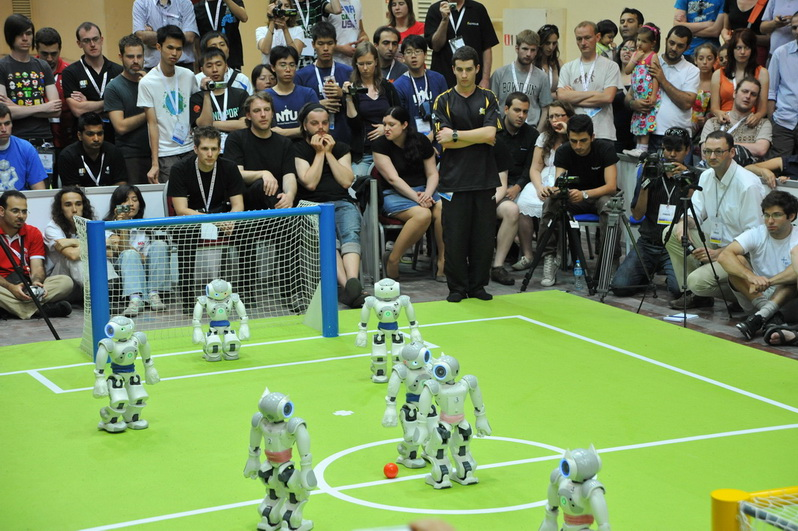
\includegraphics[width=0.6\textwidth]{Chapter1/figures/spl.jpg}
\end{figure}
   	

  }  
  
  \frame
  {
    \frametitle{Soccer}
    Humanoid League
   	\begin{figure}[t!] 
\centering
    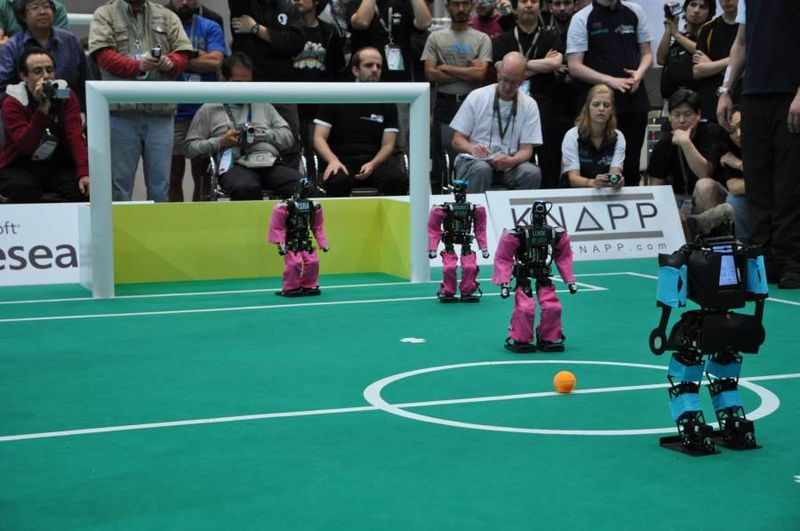
\includegraphics[height=3cm]{Chapter1/figures/kid2011.jpg}\ 
    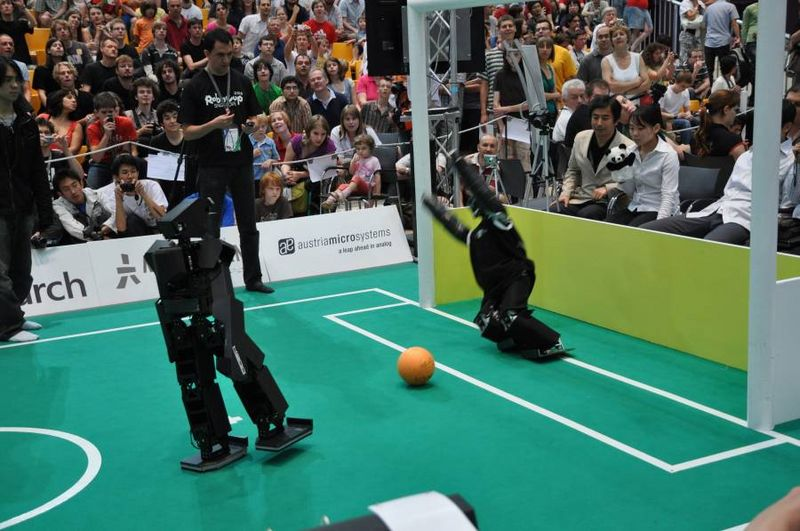
\includegraphics[height=3cm]{Chapter1/figures/teen2011.jpg}\ 
    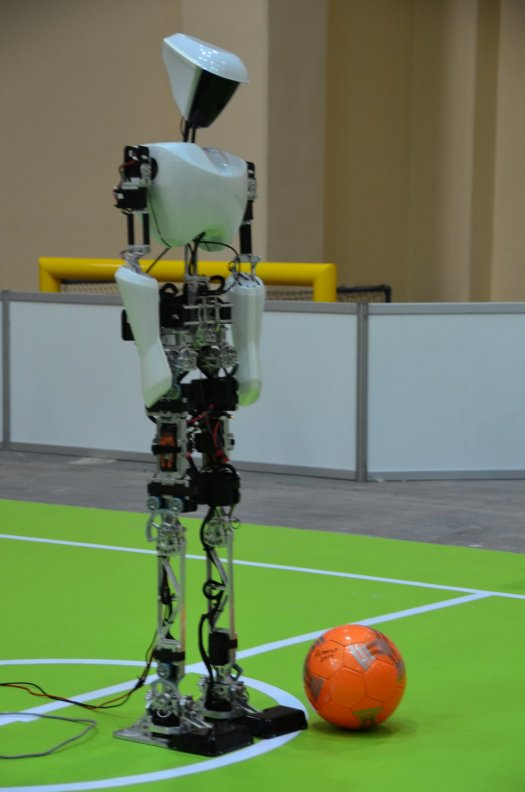
\includegraphics[height=3cm]{Chapter1/figures/adult2011.jpg}
\end{figure}
   	

  }
  
  \frame
  {
    \frametitle{Rescue}
\begin{figure}[t!]
\centering
  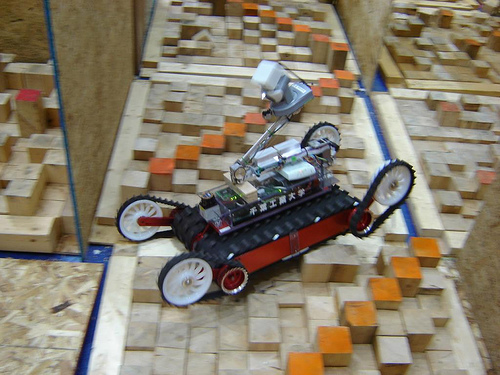
\includegraphics[width=0.6\textwidth]{Chapter1/figures/rescue.jpg}
\end{figure}
   	

  }
  
  
  \frame
  {
    \frametitle{@Home}
\begin{figure}[t!]
\centering
  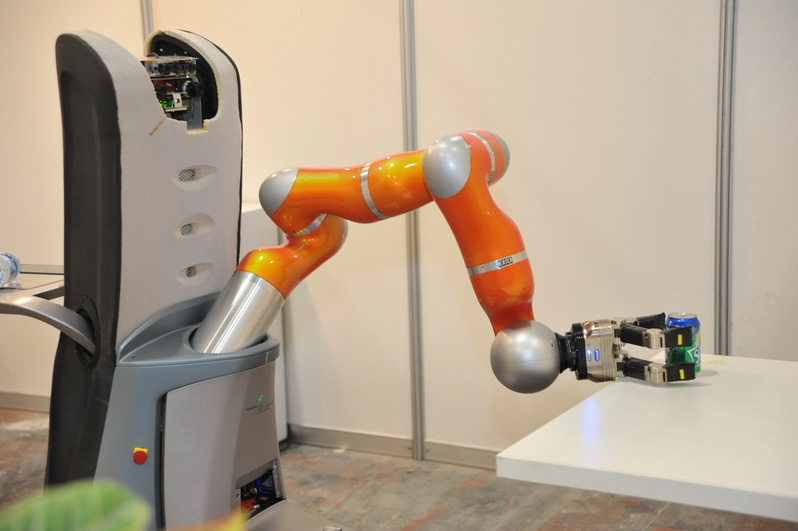
\includegraphics[width=0.6\textwidth]{Chapter1/figures/RoboCup@Home.jpg}
\end{figure}
   	

  }
  


  \subsection*{RoboCup Simulation League}
  \frame
  {
    \frametitle{Simulation League}
     \begin{itemize}[<+->]
    	\item One of the oldest leagues in RoboCup Soccer.
        \item Independently moving software players (agents).
        \item virtual field inside a computer.
        \item 2D League, 3D League.
     \end{itemize}
    

  }
  
  \frame
  {
    \frametitle{Simulation League 2D vs 3D}   
   	\begin{figure}[t!] 
\centering
    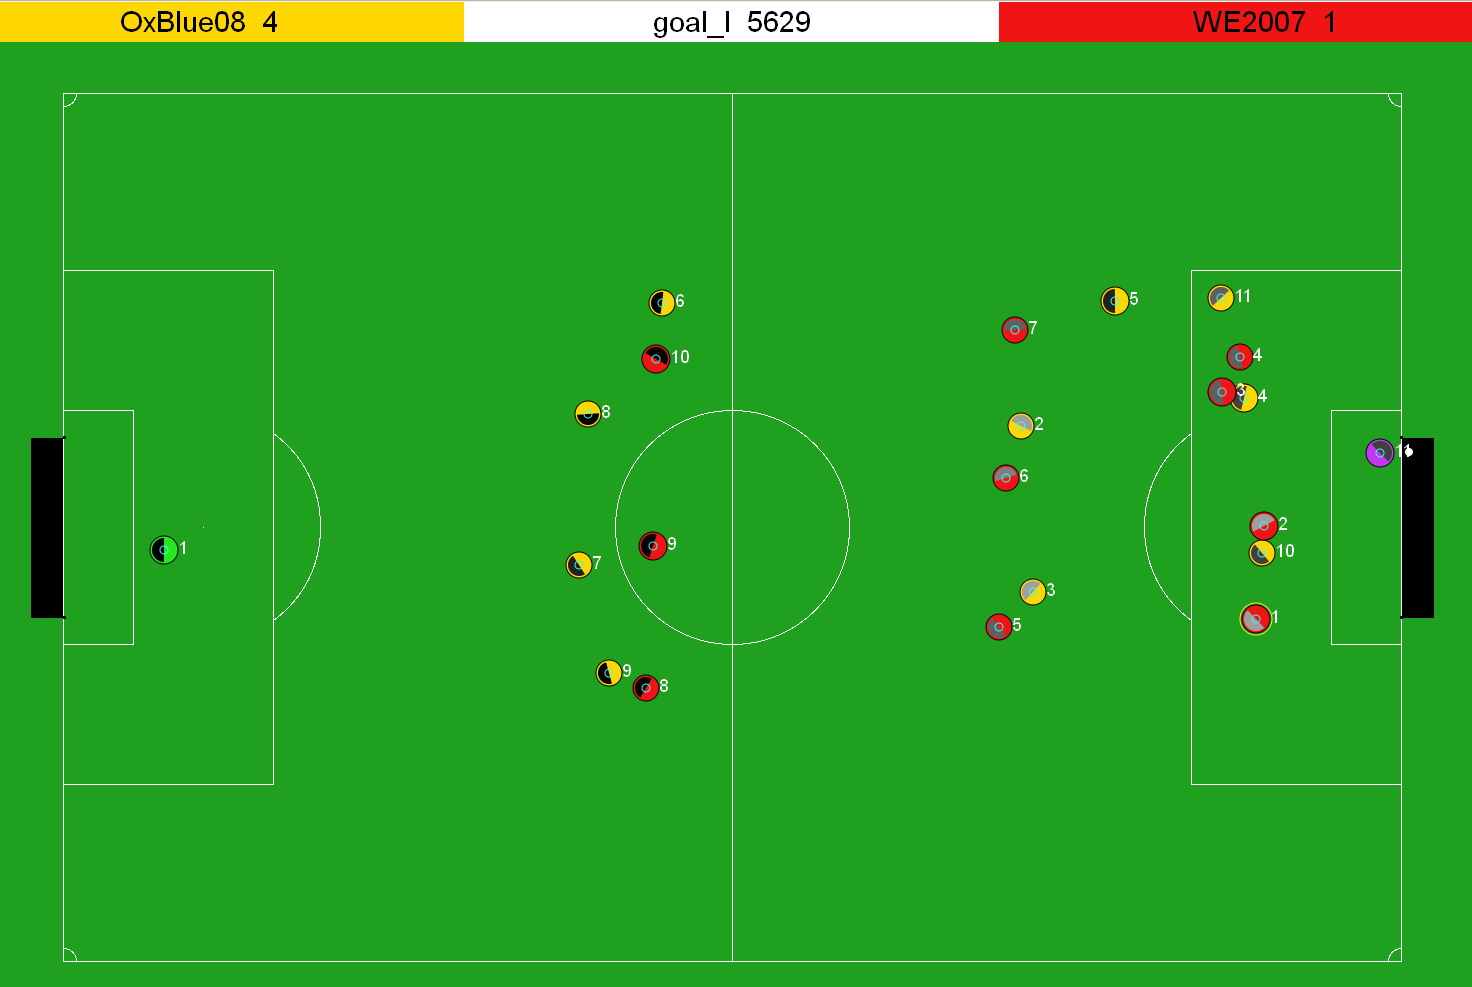
\includegraphics[height=3.5cm]{Chapter1/figures/2D.jpg}\	
    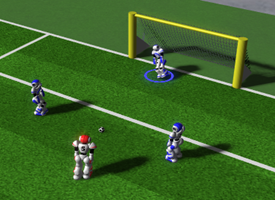
\includegraphics[height=3.5cm]{Chapter1/figures/3d.png}
\end{figure}
   	

  } 
  
  \subsection*{Simulation League 3D}
  \frame
  {
    \frametitle{3D Simulation Soccer}
    \begin{itemize}[<+->]
    \item At its beginning, spherical agent.
    \item In 2006, Fujitsu HOAP-2 robot.
    \item In 2008, Nao robot model.   
    \item \textbf{SimSpark} is used as the official Robocup 3D simulator.
    \end{itemize}
         
  }
  
  \frame
  {
    \frametitle{SimSpark}
    \begin{itemize}[<+->]
    \item \textbf{SimSpark} is a generic physics simulator system.
    \item Multiple agents in three-dimensional environment.
	\item \textit{Rcssserver3d} is the official competition environment for the RoboCup 3D Simulation League.

    \end{itemize}
         
  }
  
  \frame
  {
    \frametitle{Server's Versions}
    \begin{itemize}
    \item Version 0.6.5
    \begin{description}
    \item[Players] 9
    \item[Length] 21m
    \item[Width] 14m
    \end{description}
    
    \item Version 0.6.6
     \begin{description}
    \item[Players] 11
    \item[Length] 30m
    \item[Width] 20m
    \end{description}
    \end{itemize}
         
  }
  
  \frame
  {
    \frametitle{Soccer Field}
    \begin{figure}[t!]
\centering
  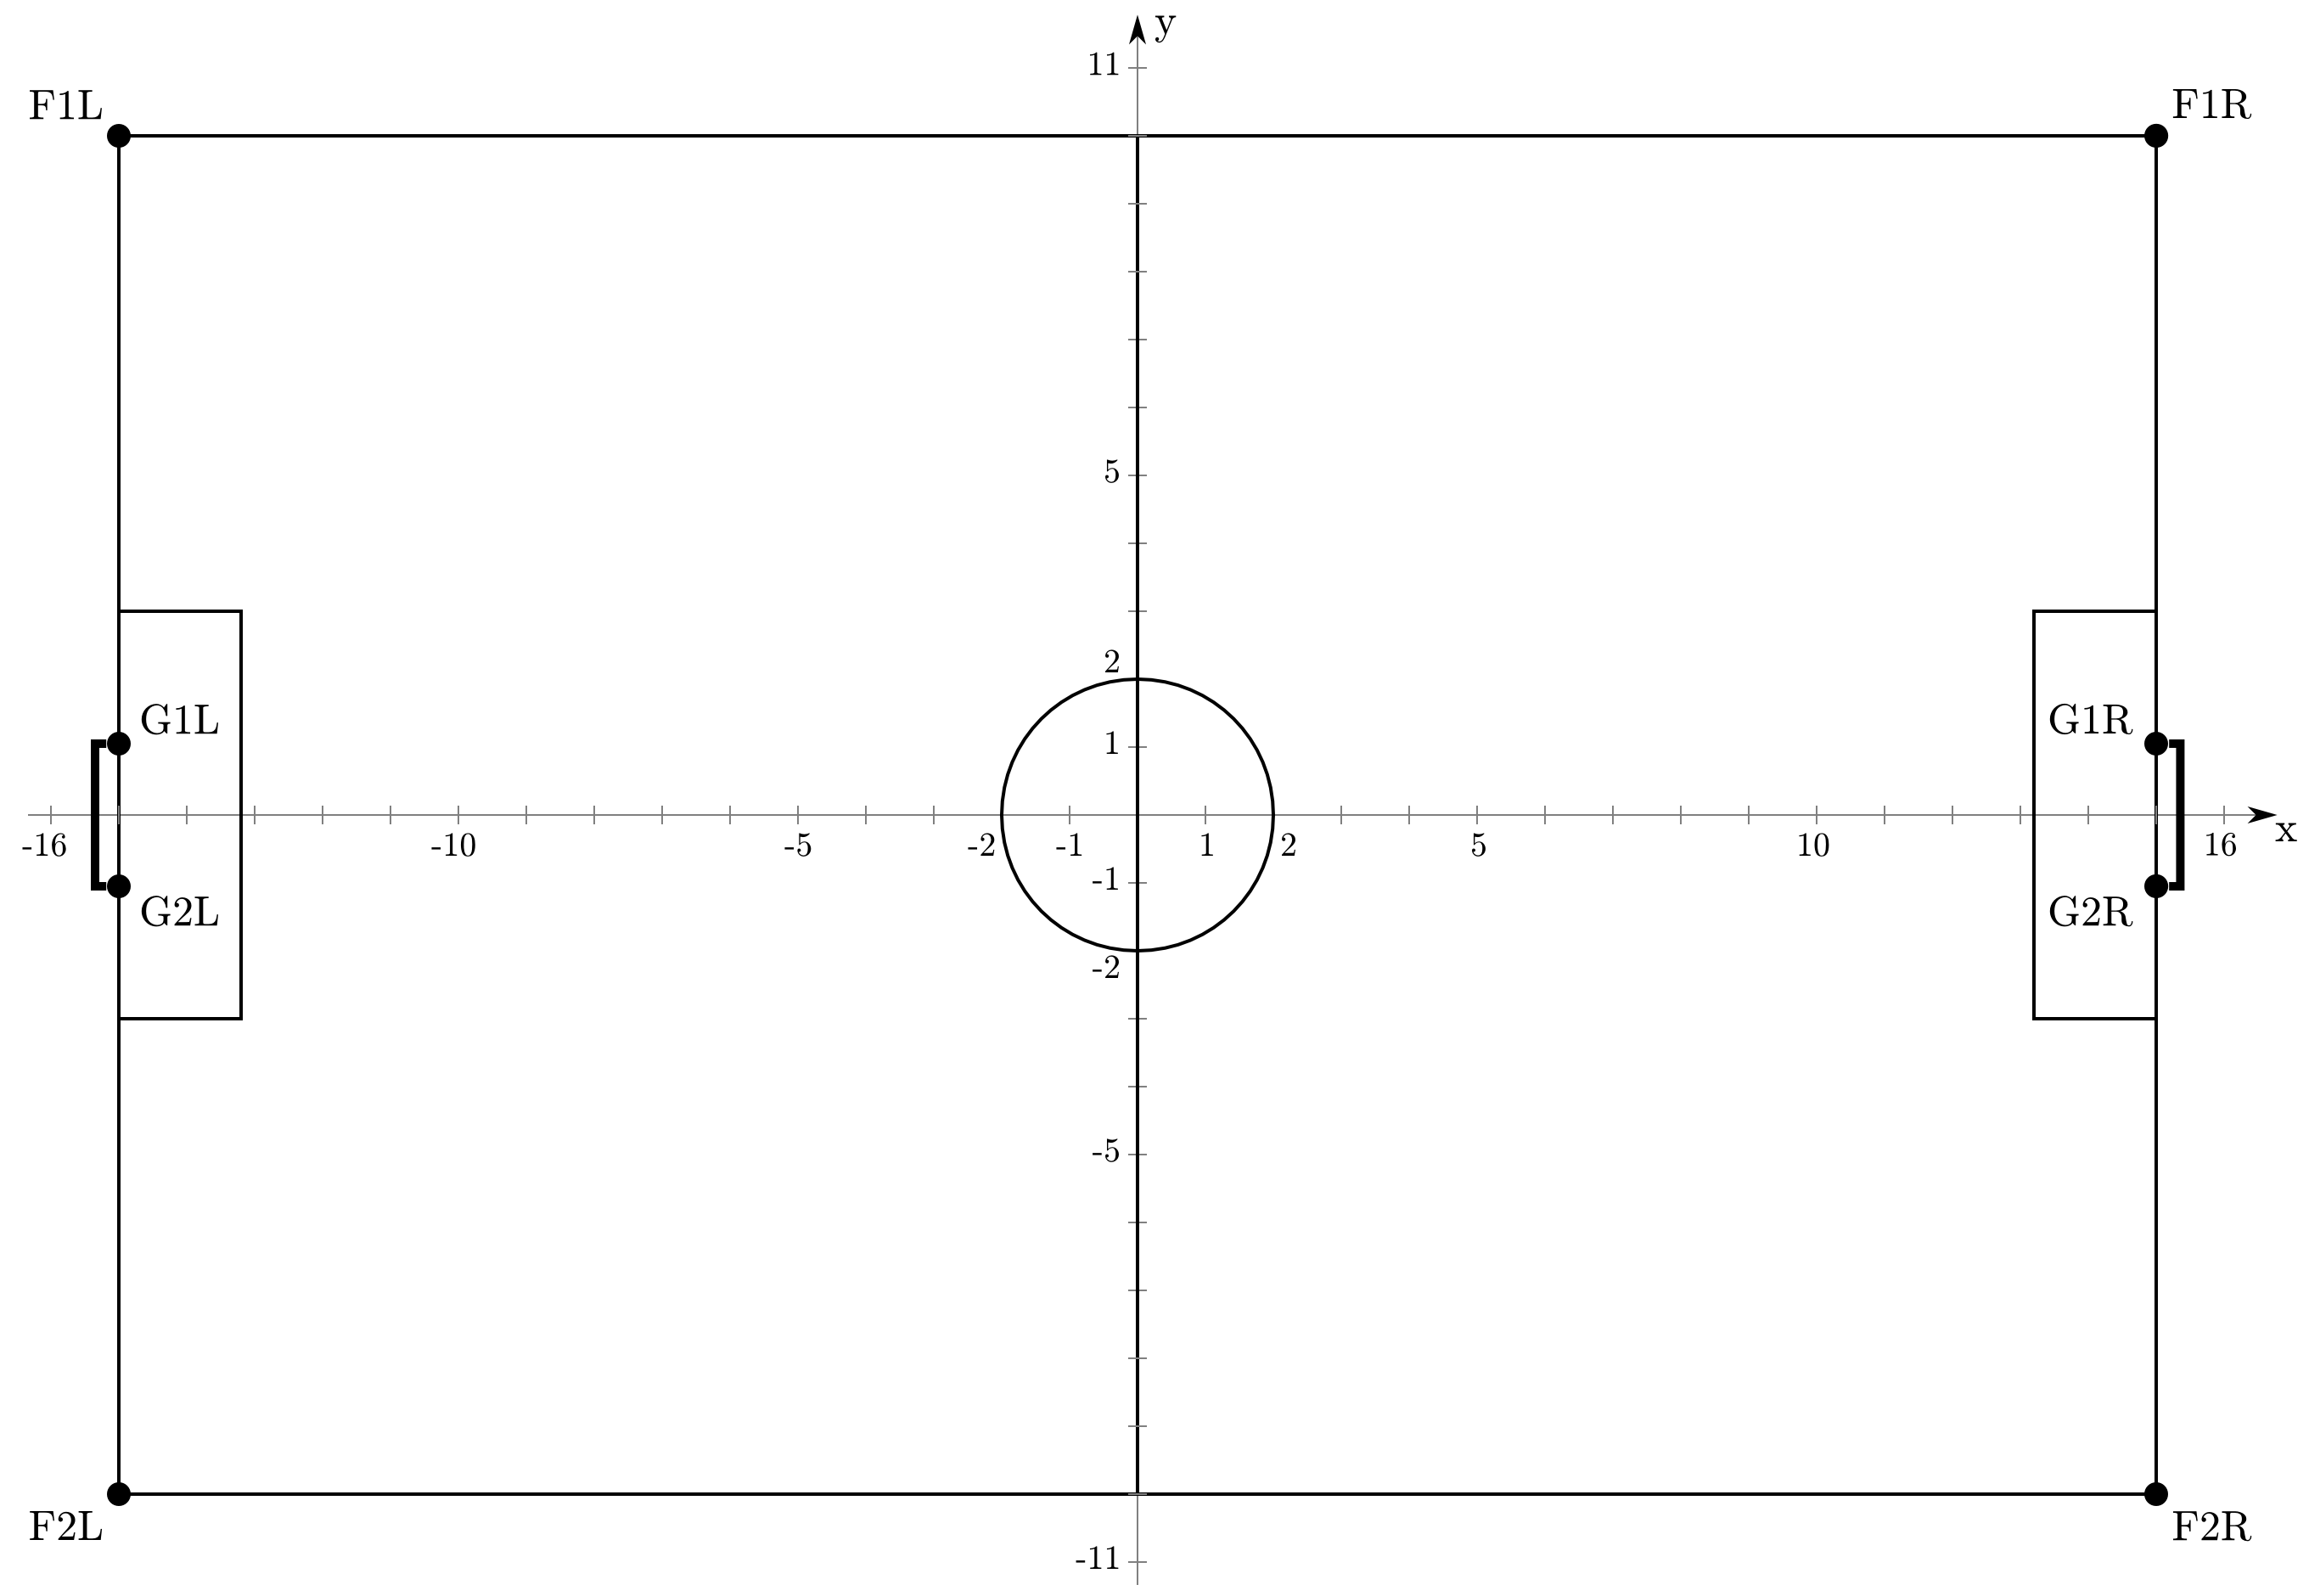
\includegraphics[width=0.8\textwidth]{Chapter2/figures/SoccerSimulation_FieldPlan.png}
\end{figure}
         
  }
  
  \frame
  {
    \frametitle{Robot Model}
    The Nao humanoid robot manufactured by Aldebaran Robotics. Its height is about 57cm and its 			weight is around 4.5kg. The simulated model comes with 22 degrees of freedom.
    \begin{figure}
\centering
  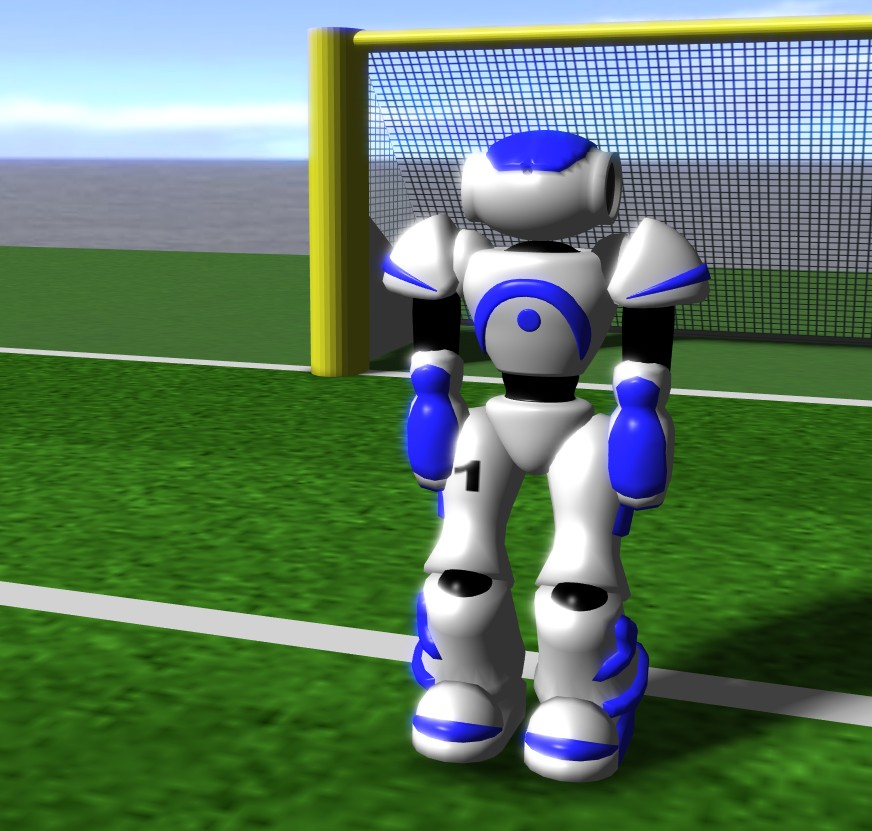
\includegraphics[trim=7cm 0cm 0cm 0cm, clip, width=0.4\textwidth]{Chapter2/figures/629px-Models-nao.jpg}
  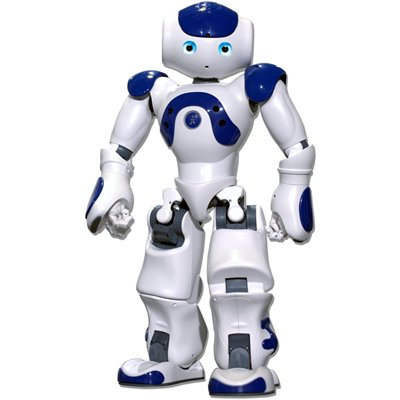
\includegraphics[width=0.4\textwidth]{Chapter2/figures/RealNao.jpg}
\end{figure}

   
  }
  
  \frame
  {
    \frametitle{Server}
    The SimSpark server hosts the process that manages and advances the simulation.
    \begin{itemize}[<+->]
	\item Simulation Cycle, 20ms
	\item Sense
	\item Think
	\item Act
    \end{itemize}
	\begin{figure}[t!]
	\centering
  		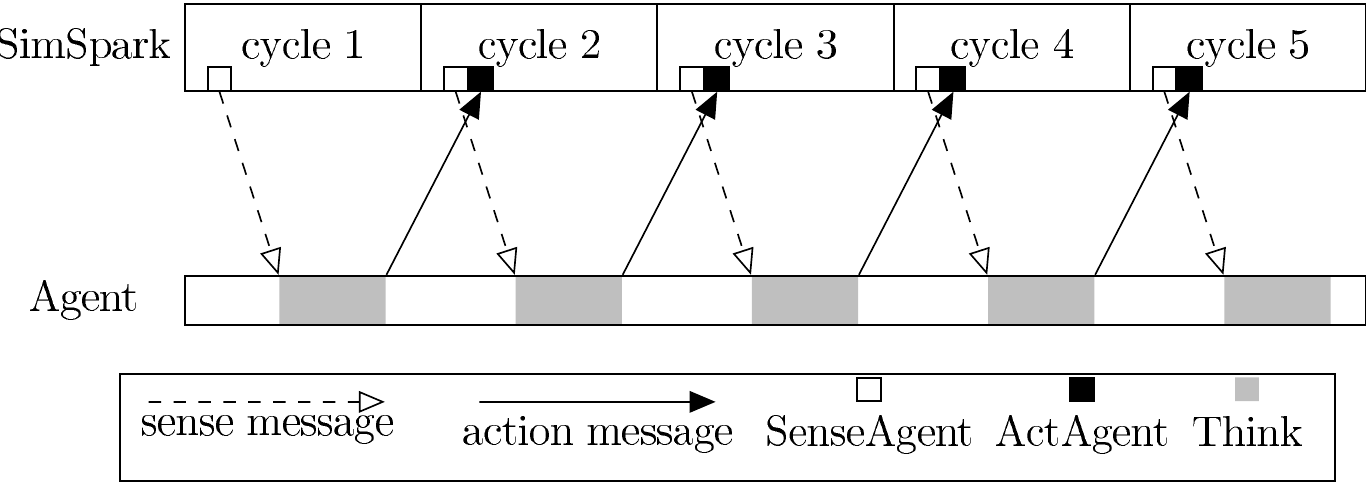
\includegraphics[width=0.6\textwidth]														{Chapter3/figures/SimulationUpdateLoopSynchronizationBetweenSimSparkAndAgent.png}
	\end{figure}
     
  }
  

  \begin{frame}
  \frametitle{Agent Perceptors}
Perceptors are the senses of an agent, allowing awareness of the agent's model state and the environment.  
  
    \begin{itemize}[<+->]
    \item HingeJoint Perceptor

    \item ForceResistance Perceptor

    \item GyroRate Perceptor

    \item Accelerometer Perceptor

    \item Vision Perceptor

    \item Hear Perceptor

    \item GameState Perceptor

    \end{itemize}
  \end{frame}
  
  \begin{frame}
    
    \frametitle{Agent Effectors}
    Effectors allow agents to perform actions within the simulation. Agents control them by sending messages to the server and the server changes the game state accordingly.

    \begin{itemize}[<+->]
     
    \item Create Effector

    \item HingeJoint Effector

    \item Synchronize Effector

    \item Init Effector

    \item Beam Effector

    \item Say Effector

    \end{itemize}
       
     
  \end{frame}
  
 \section{Player Skills}

  \subsection*{Architecture}

 \frame
  {
    \frametitle{Agents Architecture}
    
    \begin{figure}
	\centering
 	 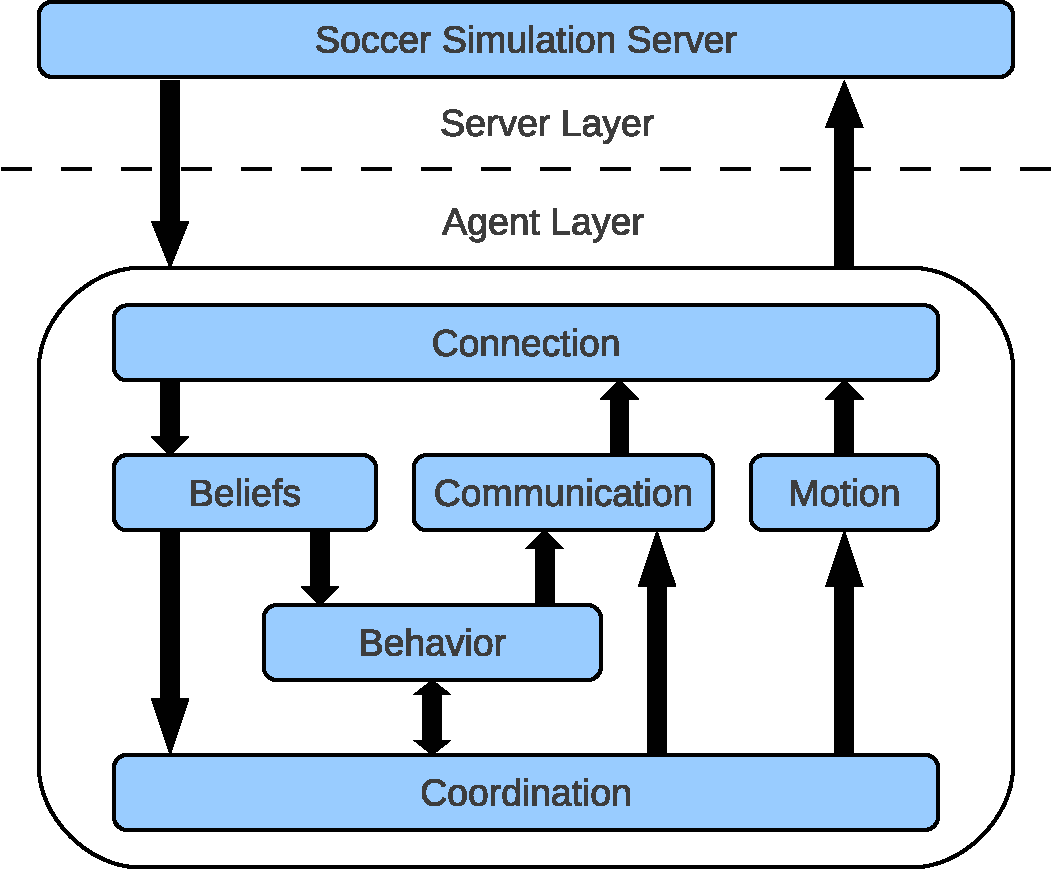
\includegraphics[width=0.7\textwidth]{Chapter3/figures/Arch.pdf}
	\end{figure}
    
  }
	


 \subsection*{General Skills}
  \frame
  {
    \frametitle{Connection}
    
	\begin{itemize}[<+->]
    \item Agent connected to the server at all times during a simulated game.
    \item Sense messages from the server every 20ms.
    \item Action messages, at the end of their think cycles.
    \end{itemize}

    
  }
  
  \frame
  {
    \frametitle{Perception}
    \begin{itemize}[<+->]
	\item Different from real robot soccer games.
    \item No raw data.
    \item Perceptor Messages.
    \item Agents update their beliefs and store sensors' data parsing these messages.
 	\end{itemize}
  
  }
  
  \begin{frame}[fragile]
  \frametitle{Perception Message Example}
  \begin{footnotesize}
  \begin{verbatim}(time (now 46.20))(GS (t 0.00) (pm BeforeKickOff))(GYR (n torso)
(rt 0.00 0.00 0.00))(ACC (n torso) (a 0.00 -0.00 9.81))(HJ (n hj
1)(ax 0.00))(HJ (n hj2) (ax 0.01))(See (G2R (pol 14.83 -11.81 1.
08))(G1R (pol 14.54 -3.66 1.12)) (F1R (pol 15.36 19.12 -1.91))(F
2R (pol 17.07 -31.86 -1.83)) (B (pol 4.51 -26.40 -6.15)) (P (tea
m AST_3D)(id 8)(rlowerarm (pol 0.18 -35.78 -21.65)) (llowerarm (
pol 0.19 34.94-21.49)))(L (pol 8.01 -60.03 -3.87) (pol 6.42 51.1
90 -39.13 -5.17))(L (pol 5.91 -39.06 -5.11) (pol 6.28-29.26 -4.8
8)) (L (pol 6.28 29.34 -4.95)(pol 6.16 -19.05 -5.00)))(HJ(n raj1
) (ax -0.01))(HJ (n raj2) (ax -0.00))(HJ (n raj3)(ax -0.00))(HJ(
n raj4) (ax 0.00))(HJ (n laj1) (ax 0.01))(HJ (n laj2) (ax 0.00)) ...
  \end{verbatim}
  \end{footnotesize}
\end{frame}


  \subsection*{Localization}
  \frame
  {
    \frametitle{Self-Localization}
    
	\begin{itemize}[<+->]
	\item Executed every three cycles (60ms).
    \item Localization uses the eight visible landmarks into the field.
    \begin{itemize}
    \item G1R, G2R, G1L, G2L
    \item F1R, F2R, F1L, F2L
    \end{itemize}
    \item Limited field of view (120 Degrees).

 	\end{itemize}

  }
  

  \frame
  {
    \frametitle{Simulated Nao's Restricted Field of View}

   \begin{figure}
	\centering
  	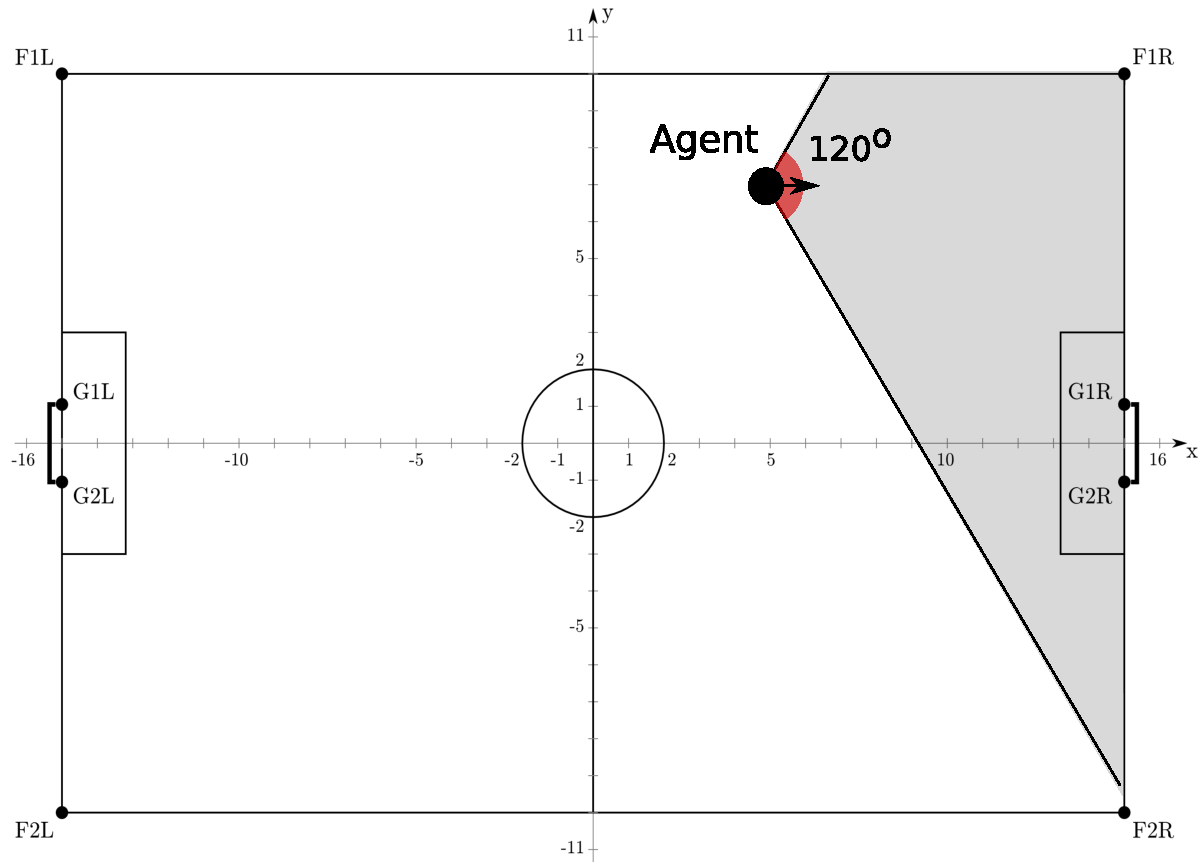
\includegraphics[width=0.8\textwidth]{Chapter3/figures/LViewAngle.pdf} 		
	\end{figure}
    
  }
    
  
  \frame
  {
    \frametitle{Self-Localization Technique}
	\begin{figure}
	\centering
  	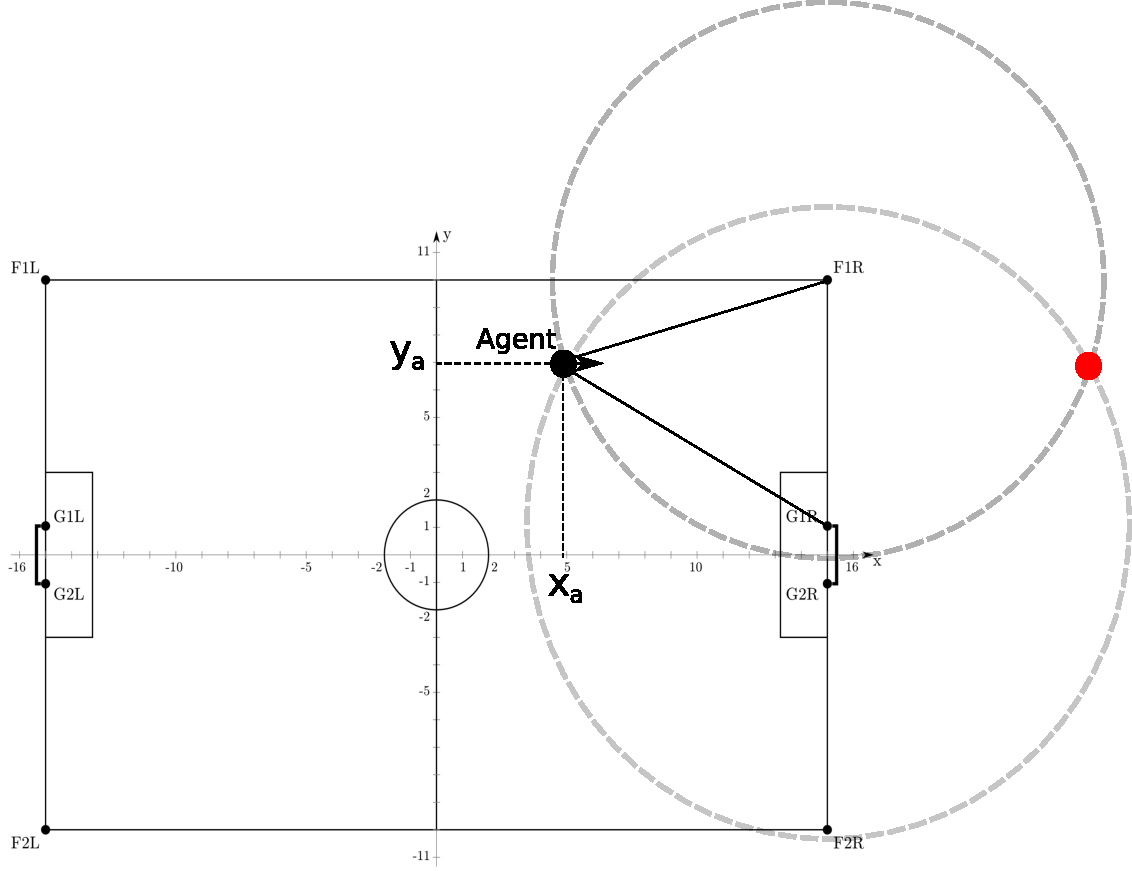
\includegraphics[width=0.8\textwidth]{Chapter3/figures/Localization.pdf}
	\end{figure}
   
    
  }
  
  \frame
  {
    \frametitle{Localization Results}
	\begin{figure}[t!]
\centering
  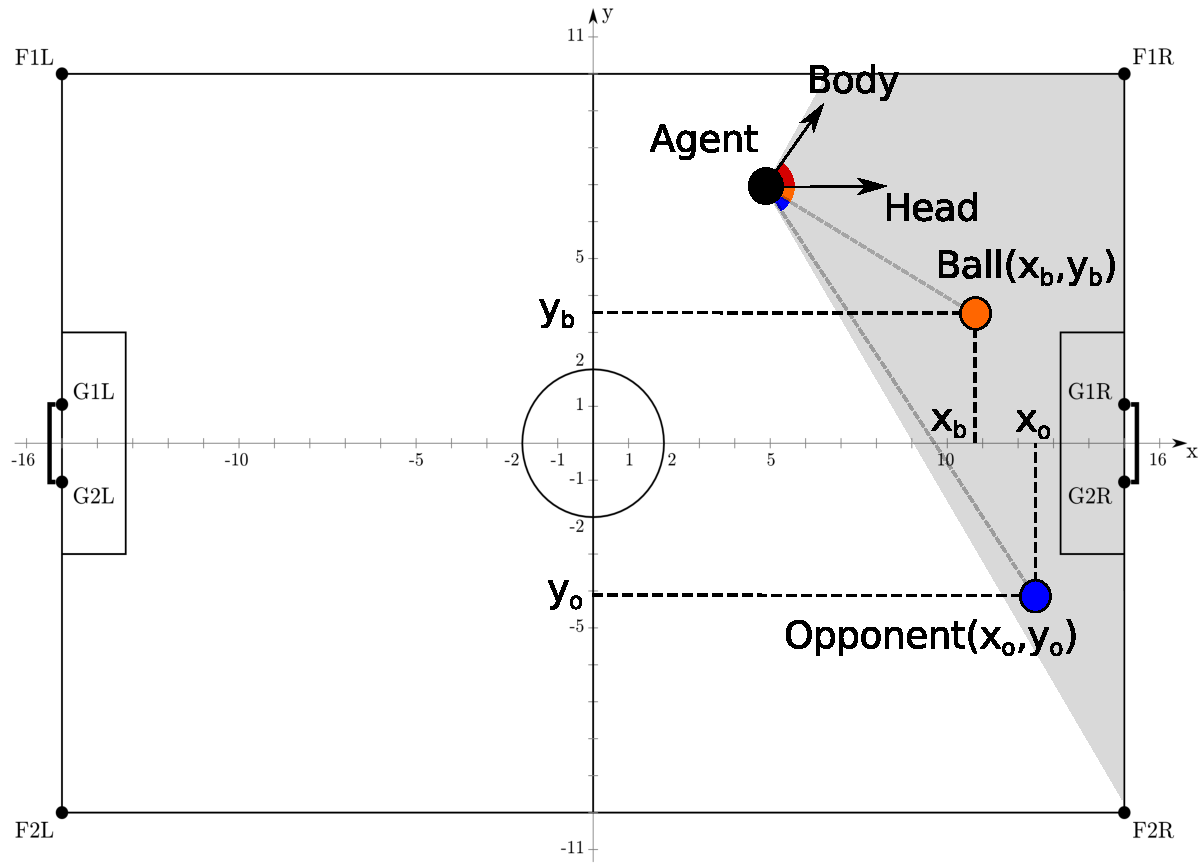
\includegraphics[width=0.8\textwidth]{Chapter3/figures/LocalizationResults.pdf}
 
\end{figure}
   
    
  }
  
  \frame
  {
    \frametitle{Localization Filtering}
    \begin{quote}
    Why a localization filtering is needed?
    \end{quote}
	\begin{itemize}[<+->]
	\item Absence of a more sophisticated probabilistic localization scheme.
	\item Temporary absences of observations from self-localization.
	\item Noisy observations.   
	\item Filter incoming observations.
	\item Filter incoming observations.
	\end{itemize}
	Filtering is applicable for ball and self localization.
   
    
  }
 
  \frame
  {
    \frametitle{Localization Filtering Algorithm}
\begin{algorithm}[H]
\caption{Localization Filtering}
\label{LocalizationFiltering}
\begin{algorithmic}[1]
\begin{footnotesize}
\STATE {\bf Input: }$LastEstimate$
\STATE {\bf Output: }$FilteredLocation$
\STATE $Queue$: a FIFO queue storing the $MaxSize$ (default=10) most recent estimates
\STATE 
\IF{$size(Queue) = 0$}
\STATE $Queue.Add(LastEstimate)$
\ELSIF{$LastEstimate \not\approx AverageLocation(Queue)$}
\STATE $Queue.Remove()$
\ELSE 
\IF{$size(Queue) = MaxSize$}
\STATE $Queue.Remove()$
\ENDIF
\STATE $Queue.Add(LastEstimate)$
\ENDIF
\RETURN $AverageLocation(Queue)$
\end{footnotesize}
\end{algorithmic}
\end{algorithm}
   
    
  }
  
  
  \subsection*{Motions and Movement}
  
  
  \frame
  {
    \frametitle{Nao's Anatomy}
    The simulated Nao robot comes with 22 degrees of freedom, corresponding to 22 hinge
joints.
\begin{figure}
\centering
  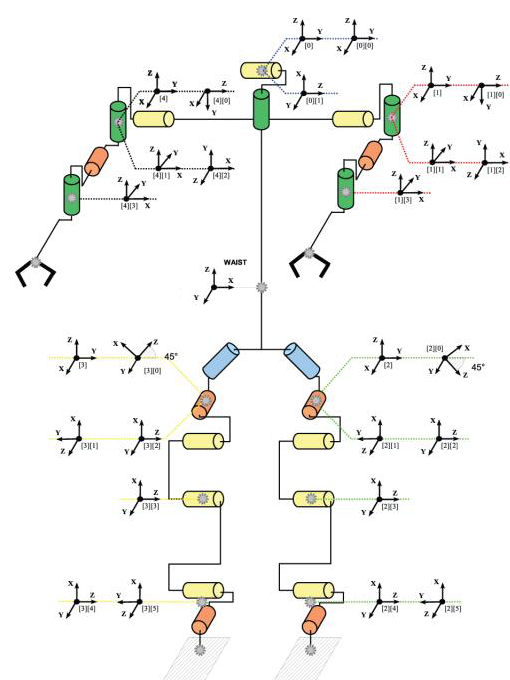
\includegraphics[width=0.3\textwidth]{Chapter3/figures/Models_NaoAnatomy.png}
\end{figure}

  }
  
  \frame
  {
    \frametitle{Motion and Movement}
	\begin{itemize}[<+->]
	\item In robotics, a complex motion is commonly defined as a sequence of timed joint poses.
	\item A pose is a set of values for every joint in the robot's body or in a specific kinematic chain at a given time.
	 \[
	Pose(t)= \lbrace J_{1}(t), J_{2}(t), \ldots ,J_{n}(t) \rbrace
	\]  
	\end{itemize} 
	 


  }
  
  \begin{frame}[fragile]
  \frametitle{XML-Based Motion Files}
  \begin{tiny}
  \begin{verbatim}<phase name="Start" next="Phase1">
   <effectors>
      Joint Values
   </effectors>
   <duration>duration</duration>
</phase>

<phase name="Phase1" next="Phase2">
   <effectors>
      Joint Values
   </effectors>
   <duration>duration</duration>
</phase>

<phase name="Phase2" next="Phase1">
   <effectors>
      Joint Values
   </effectors>
   <duration>duration</duration>
   <finalize>Final</finalize>
</phase>

<phase name="Final">
   <effectors>
      Joint Values
   </effectors>
   <duration>duration</duration>
</phase>
  \end{verbatim}
  \end{tiny}
  
  \putat{200}{30}{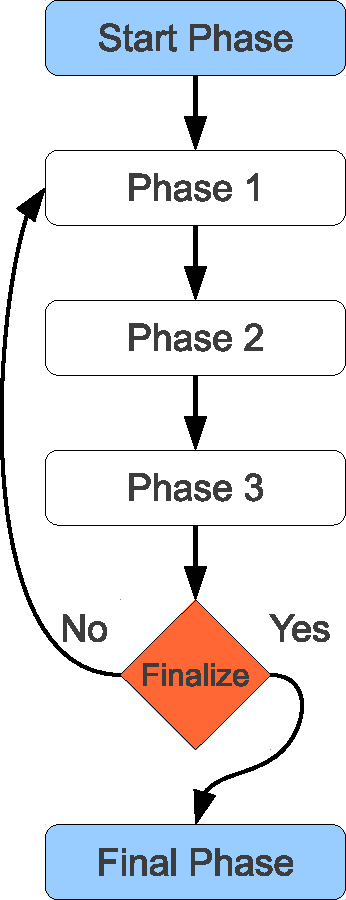
\includegraphics[width=0.2\textwidth]{Chapter3/figures/MotionSequence.pdf}}
  
\end{frame}


\frame
  {
    \frametitle{XML-Based Motion Controller}
    \frametitle{Motion and Movement}
	\begin{itemize}[<+->]
	\item To generate motions.
	\item Velocity computation is required.
	\item This velocity is computed as follows:
	\[
Joint Velocity = \cfrac{Desired Joint Value - Current Joint Value}{PhaseDuration}
\]
	\end{itemize}

  }
  
  
   
 \begin{frame}[fragile]
  \frametitle{Text-Based Motion Files}
  \begin{footnotesize}
  \begin{verbatim}#WEBOTS_MOTION,V1.0
LHipYawPitch,LHipRoll,LHipPitch,LKneePitch,LAnklePitch,...
00:00:000,Pose1,0,-0.012,-0.525,1.05,-0.525,0.012,0,...
00:00:040,Pose2,0,-0.011,-0.525,1.05,-0.525,0.011,0,...
00:00:080,Pose3,0,-0.009,-0.525,1.05,-0.525,0.009,0,...
00:00:120,Pose4,0,-0.007,-0.525,1.05,-0.525,0.007,0,...
00:00:160,Pose5,0,-0.004,-0.525,1.05,-0.525,0.004,0,...
00:00:200,Pose6,0,0.001,-0.525,1.051,-0.525,-0.001,0,...
00:00:240,Pose7,0,0.006,-0.525,1.05,-0.525,-0.006,0,...
00:00:280,Pose8,0,0.012,-0.525,1.05,-0.525,-0.012,0,...
00:00:320,Pose9,0,0.024,-0.525,1.05,-0.525,-0.024,0,...
\end{verbatim}
  \end{footnotesize}
\end{frame}

\frame
  {
    \frametitle{Text-Based Motion Controller}
    
Parameters that can be modified:
\begin{itemize}[<+->]
	\item Duration, time between poses in simulation cycles.
	\item PoseStep, step for advancing from pose to pose.

\item The desired velocity of each joint $i$ is computed by:
\[
JointVelocity_i = \cfrac {Desired Joint Value_i - Current Joint Value_i} {Duration \times CycleDuration}
\]
\end{itemize}

  }
  
  
\frame
  {
    \frametitle{Dynamic Motion Elements}
    \begin{itemize}[<+->]
    \item Walk Leaning 
    \item Walk Slowdown
    \item Dynamic Turn
    \end{itemize}

  }
  
  \frame
  {
	\begin{description}
	\item[X-Axis] Gain factor
	\item[Y-Axis] Agent turn
\end{description}	    
    
    \frametitle{Dynamic Turn Example}
    \begin{figure}
	\centering
 	 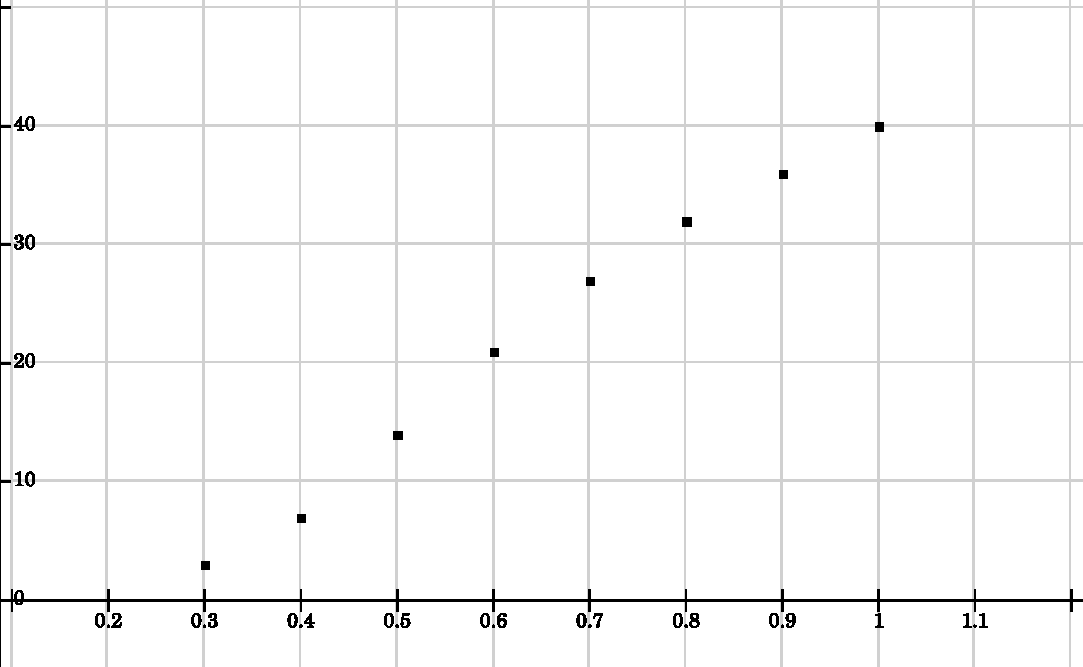
\includegraphics[width=0.8\textwidth]{Chapter3/figures/DynamicTurn.pdf}
	\end{figure}
  }
  
  \frame
  {

\frametitle{Walk Leaning}
  \begin{figure}[t!]
\centering
  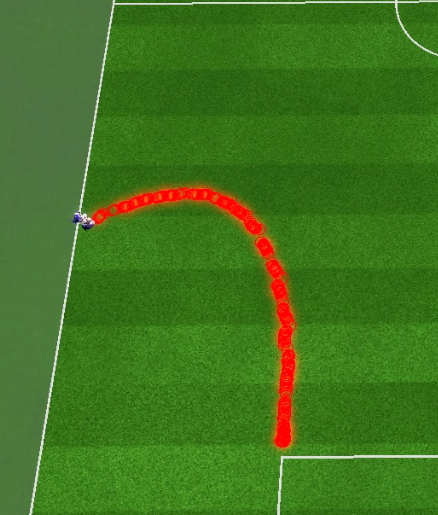
\includegraphics[height=6cm]{Chapter3/figures/leanLeft.png}\quad
  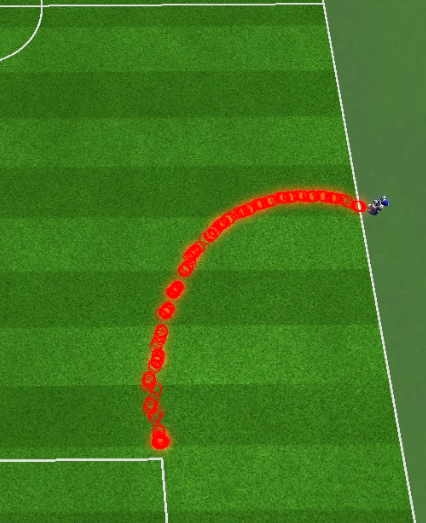
\includegraphics[height=6cm]{Chapter3/figures/leanRight.png}
\end{figure}
  }
  
  \subsection*{Actions}
  \begin{frame}

    \frametitle{Actions}
    Actions are split into groups in terms of their complexity:
    \begin{itemize}[<+->]
    \item Basic Actions
    \item Complex Actions
    \end{itemize}
  
  \end{frame}
  
  \begin{frame}
    \frametitle{Simple Actions}
	\begin{itemize}[<+->]
    \item Look Straight
    \item Scan
    \item Pan Head
    \item Track Object
    \item Track Moving Object
    \item Find Opponent�s Goals
	\item Look For Ball
	\item Turn To Ball
	\item Turn To Localize
	\item Stand Up
	\item Prepare for Kick
    \end{itemize}

  \end{frame}
  
  
  \begin{frame}
    \frametitle{Complex Actions}
    \begin{itemize}[<+->]
	\item Avoid Obstacles
    \end{itemize}
\begin{figure}
\centering
  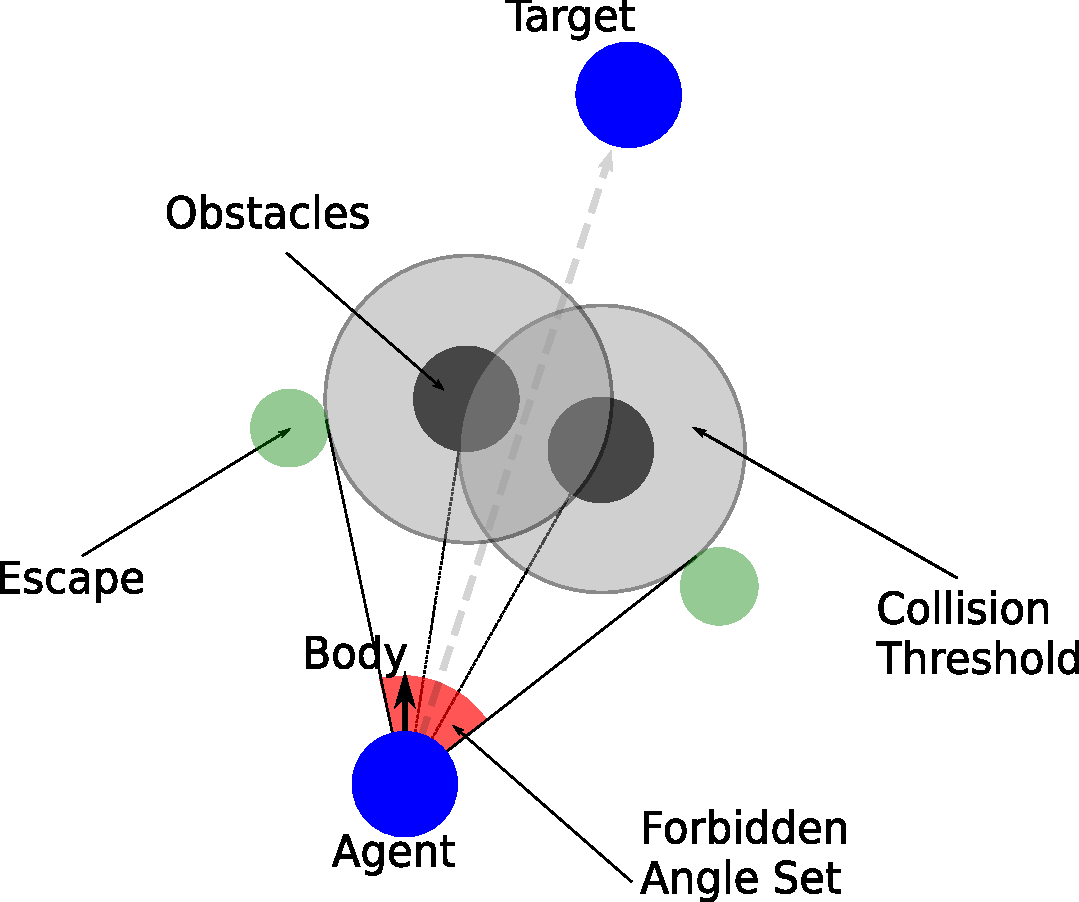
\includegraphics[width=0.6\textwidth]{Chapter3/figures/ObstacleAvoidance.pdf}
\end{figure}

\end{frame}

\begin{frame}
    \frametitle{Complex Actions}
	\begin{itemize}[<+->]
	\item On Ball Action	
    \item Walk to Ball
\begin{figure}[H]
\centering
  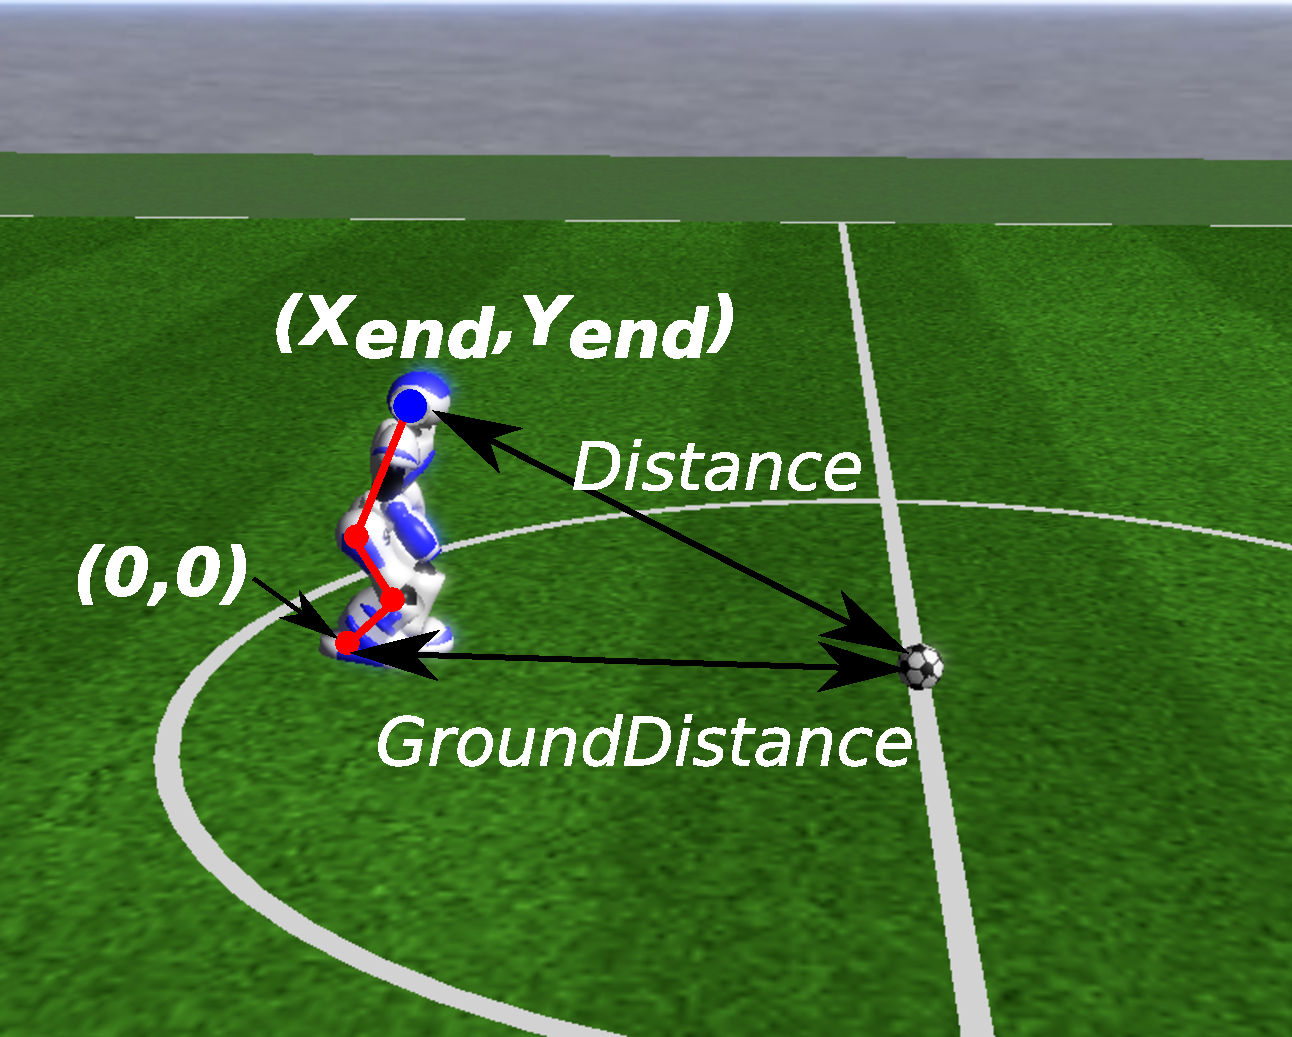
\includegraphics[trim=0cm 4cm 3cm 4cm,clip,width=0.6\textwidth]{Chapter3/figures/2dkinematics.pdf}
\end{figure}

	\end{itemize}

  \end{frame}
  
  
  \begin{frame}
    \frametitle{Complex Actions}
	\begin{itemize}[<+->]
	\item Walk To Direction 	
	\item Dribble Ball To Direction
	\item Walk to Coordinate
	\begin{figure}[H]
\centering
  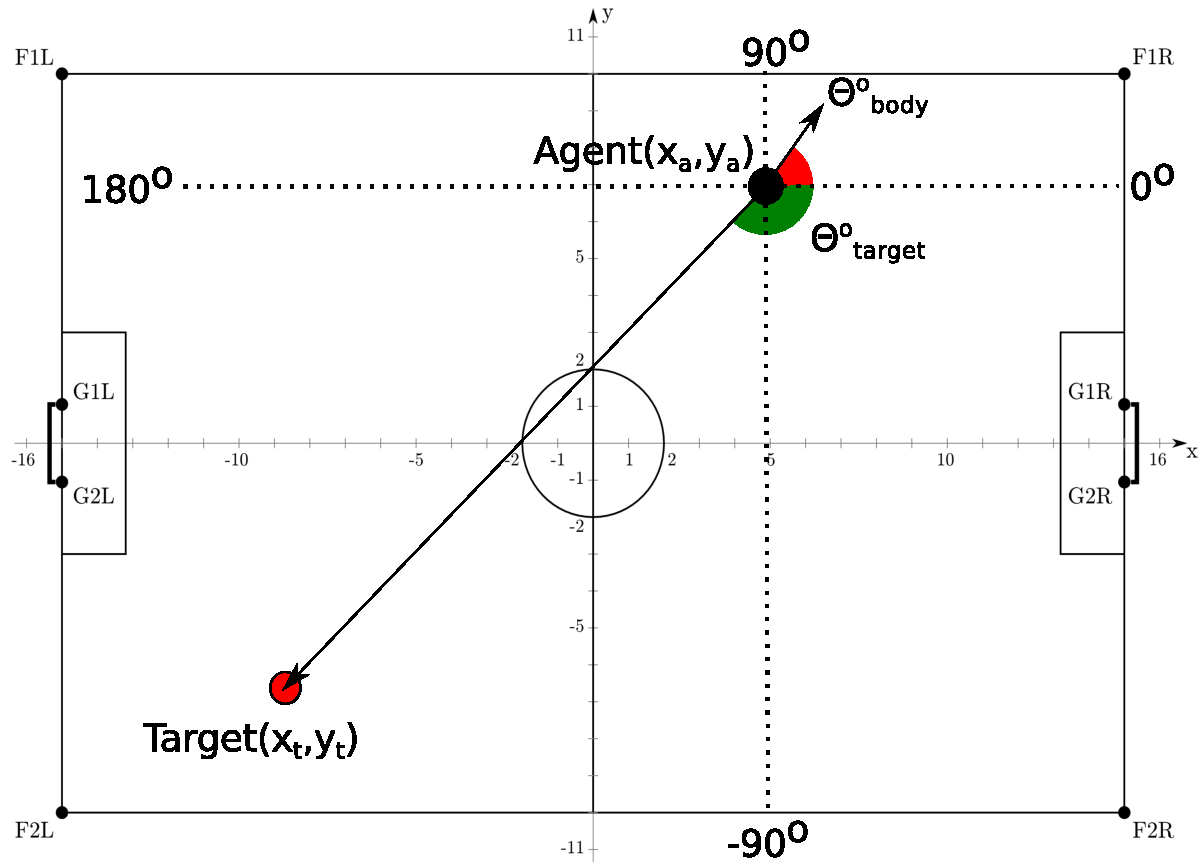
\includegraphics[trim=0cm 0cm 0cm 0cm,clip,width=0.5\textwidth]{Chapter3/figures/GoToPos.pdf}
\end{figure}
	
	
    \end{itemize}

  \end{frame}



  \subsection*{Communication}

\begin{frame}

    \frametitle{Communication Restrictions}  
  \begin{itemize}[<+->]       
    \item Maximum distance of 50 meters.   
    \item Maximum length of 20 ASCII characters.
    \item Only one message can be heard at any given time.
    \item Messages from the same team can be heard only every other cycle.
    \end{itemize}

\end{frame}
  
  \begin{frame}

    \frametitle{Communication Protocol}

    \begin{itemize}[<+->]
        
    \item Every time slice of the protocol has an associated integer label which indicates the uniform number of the player able to send its message at that slice. 
    \begin{figure}[H]
\centering
  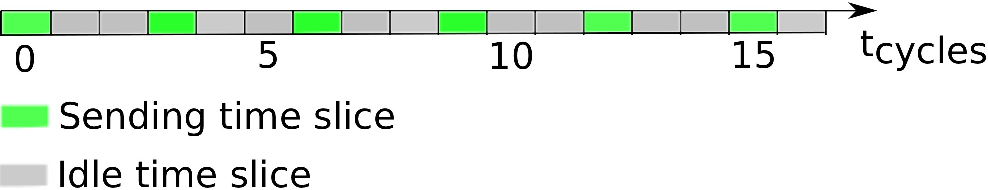
\includegraphics[width=0.5\textwidth]{Chapter3/figures/MAC.pdf}
\end{figure}   
    \item This label starts at $1$ and grows by $1$ every time a player sends a message.
    \item Every player can receive reliably the messages from all teammates every 540ms (27 cycles) for a team of 9 players or every 660ms (33 cycles) for a team of 11 players.
    \end{itemize}

\end{frame}
    
 
  \section{Team Coordination}
  
  \subsection*{Protocol}
  
 
  \begin{frame}
  
 	 \frametitle{Team Coordination}
 	 
 	 \begin{itemize}[<+->]
 	 \item Dynamic determination of individual behaviors for each agent. 
 	 \item Executed only by one agent, the coordinator.
 	 \item All players communicate their beliefs to the coordinator.
 	 \item Coordinator sends back to the players the computed actions.
 	 \begin{figure}[t!]
\centering
  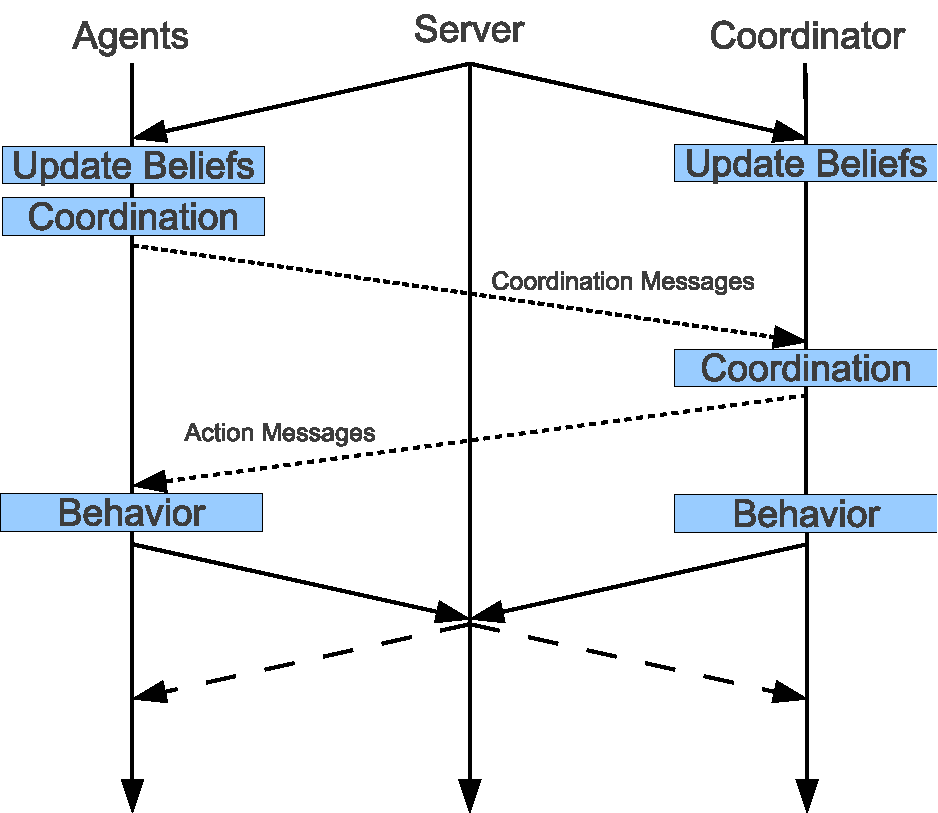
\includegraphics[width=0.3\textwidth]{Chapter4/figures/CoordinationCycle.pdf}
\end{figure}
 	 \end{itemize}
 	 
 	 \end{frame}
 	 
 	 
  \begin{frame}
  
 	 \frametitle{Coordination Phases}
 	 \begin{itemize}[<+->]
 	 \item Update Coordination Beliefs
 	 \item Determine Coordination Subsets
 	 \begin{itemize}
		\item \textit{Goalkeeper}: one player, the goalkeeper
		\item \textit{Inactive}: players fallen on the ground or players with lost self-location
		\item \textit{Active}: three players, the ones closest to the ball
		\item \textit{Support}: all remaining players
	 \end{itemize}
 	 \item Determine Active Positions
 	 \item Coordinate Active Players
 	 \item Generate Team Formation
 	 \item Assign Team Roles
 	 \item Determine Support Positions
 	 \item Coordinate Support Players
 	 \end{itemize}	 
 	 \end{frame}
 	 
 	 
 	 \begin{frame}
  
 	 \frametitle{Coordination Modes}

Coordination is not a static procedure and may change dynamically during different game states. There are three modes of team coordination:
\begin{itemize}[<+->]
\item Active Mode
\item Support Mode
\item Wait Mode
\end{itemize}

\end{frame}


\subsection*{Coordination and Communication}

\begin{frame}
 	 \frametitle{Message Types and Communication}
 	 There are several types of messages, each one of them having different functionality and serving a specific purpose.
\begin{itemize}[<+->]
\item Init Message 

\item Start Message 

\item Coordination Message  

\begin{itemize}

\item Type C, position, ball position.

\item Type L, position.

\item Type B, ball position in relation to body. 

\item Type X, empty messages.  
 
\end{itemize}

\item End Message 

\item Action Message 

\end{itemize}

\end{frame}




\begin{frame}
 	 \frametitle{Messaging Protocol}
 	 \begin{figure}[t!]
\centering
  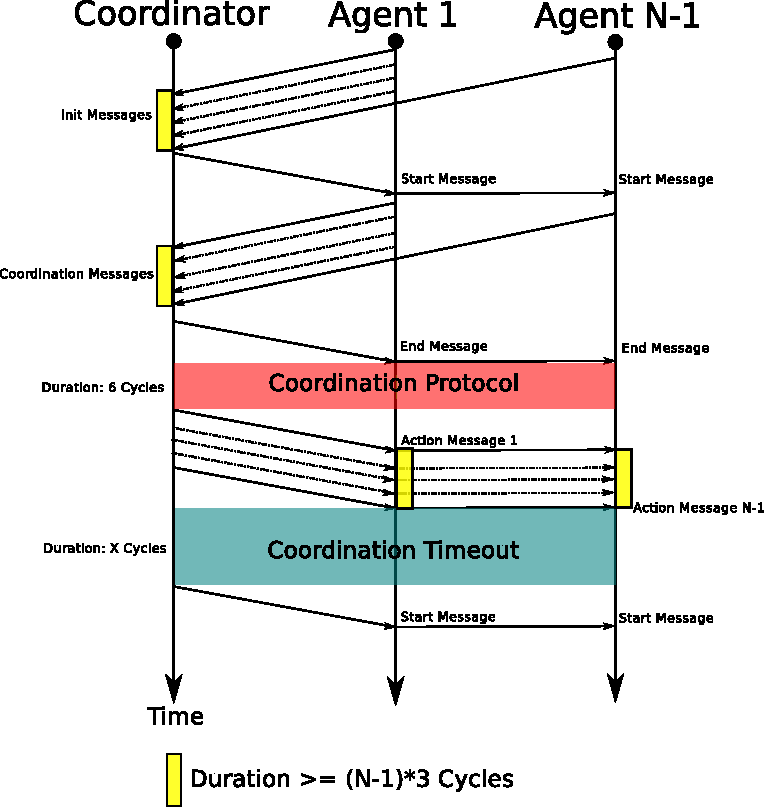
\includegraphics[width=0.6\textwidth]{Chapter4/figures/CoordComm.pdf}
\end{figure}
 	 
\end{frame}





\subsection*{Coordination Beliefs Update}


\begin{frame}
 	 \frametitle{Coordination Beliefs}
	 Coordination need to have a good knowledge about the world state. 	 
 	 \begin{itemize}[<+->]
 	 \item Global ball position
 	 \item Agents' distances from ball
 	 \item Agents' positions
 	 \end{itemize}
 	 
 	 
\end{frame}

\begin{frame}
 	 \frametitle{Estimated Ball Position}
	 \begin{figure}[t!]
\centering
  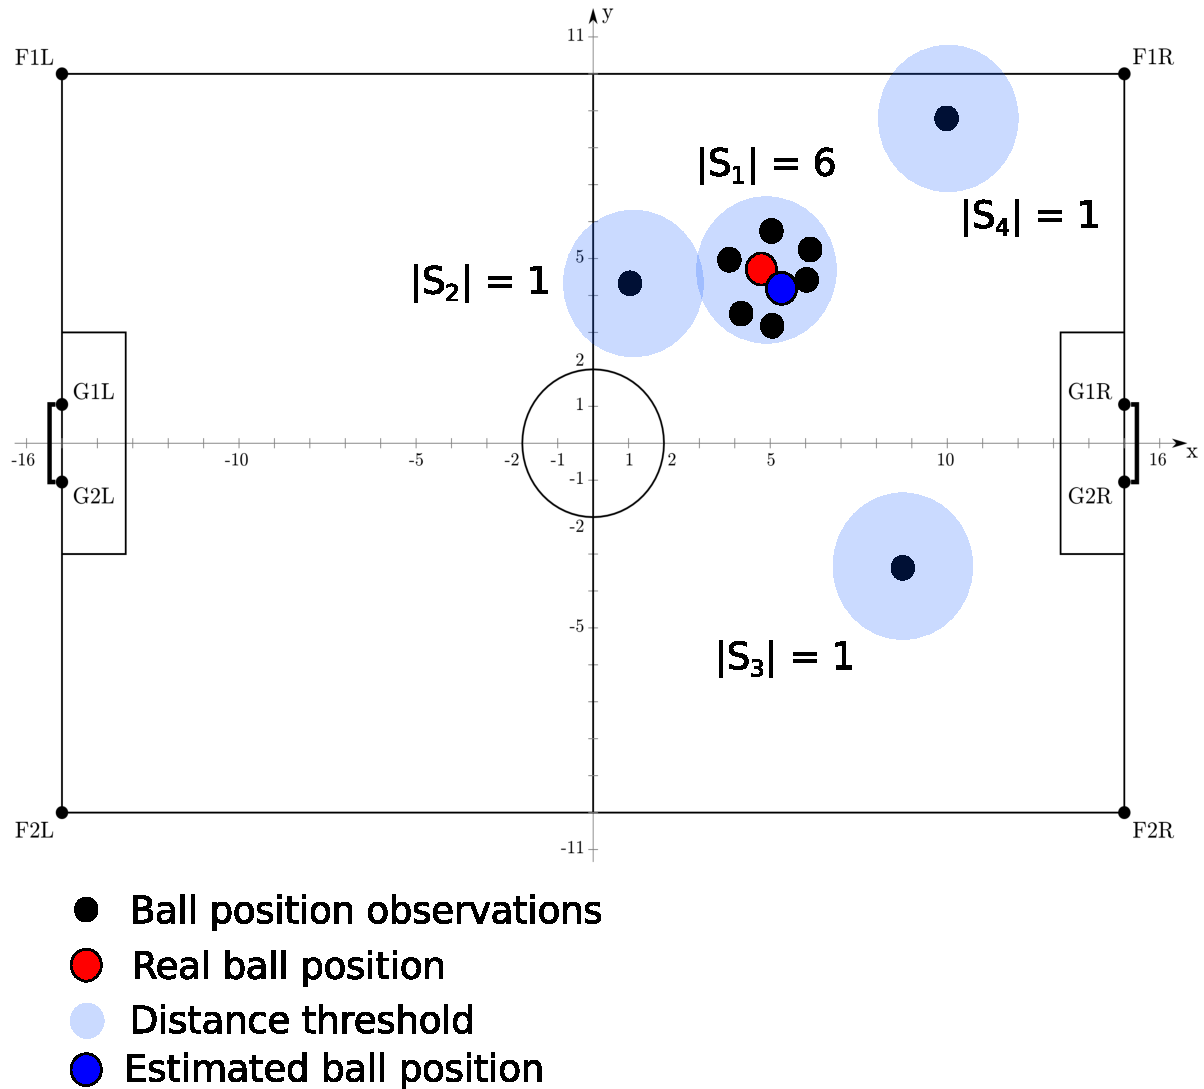
\includegraphics[width=0.5\textwidth]{Chapter4/figures/Ball.pdf}
\end{figure}
\begin{align*}
{\bf Global Ball Belief} = \sum_{i=1}^m \frac {w(s_i)} {\sum_{k=1}^m w(s_k)} \sum_{o_{ij} \in s_i} \cfrac{o_{ij}}{|s_i|}
\end{align*}
 	 	 
\end{frame}



\subsection*{Determination of Coordination Subsets}
\begin{frame}
 	 \frametitle{Coordination Splitter}
 	 \begin{figure}[t!]
\centering
  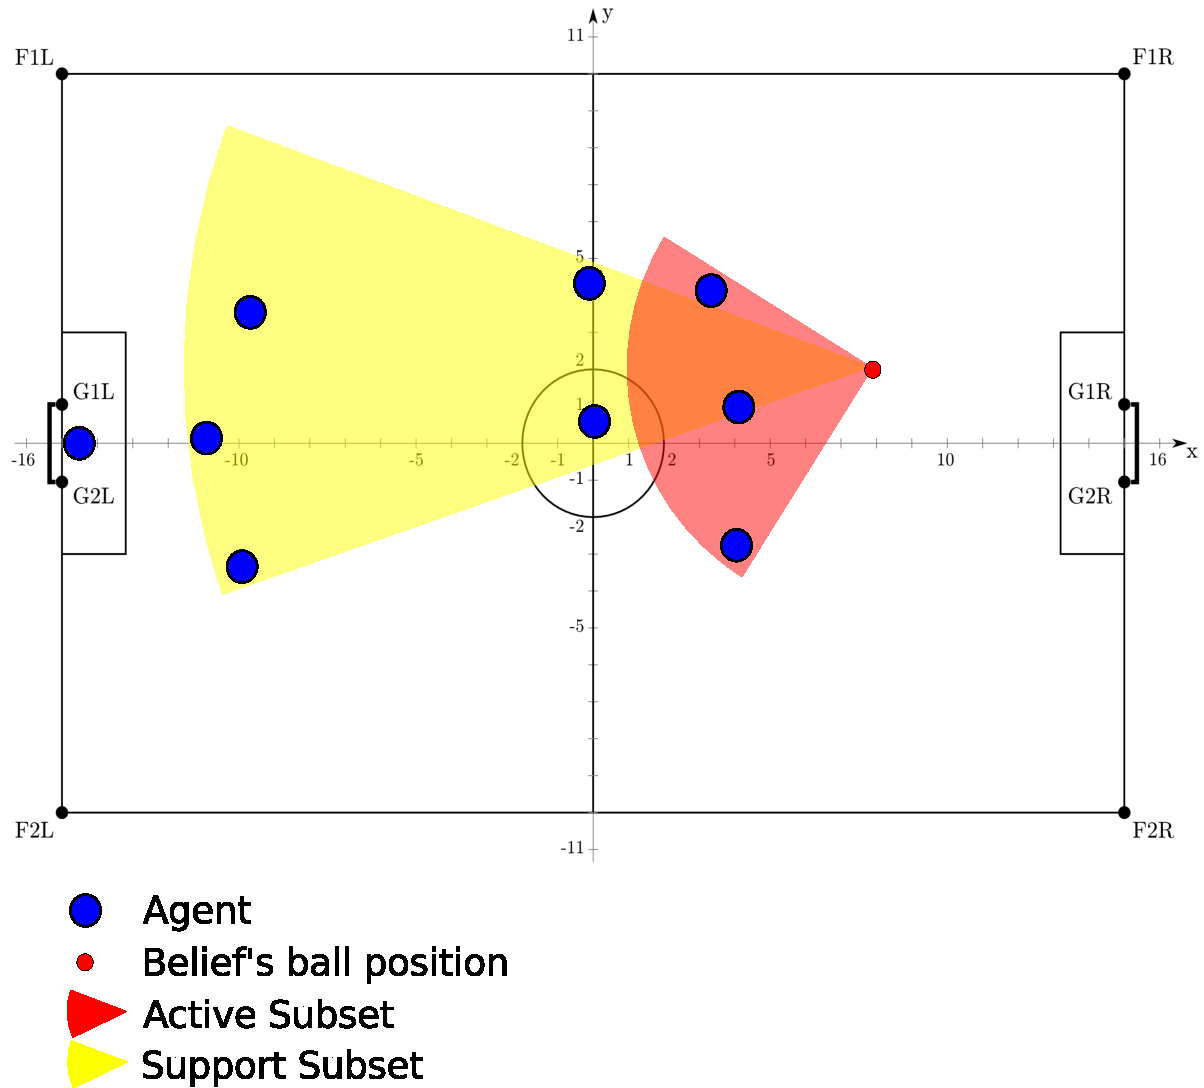
\includegraphics[width=0.6\textwidth]{Chapter4/figures/Splitter.pdf}
\end{figure}
\end{frame}





\subsection*{Soccer Field Utility Fuction}
\begin{frame}
 	 \frametitle{Soccer Field Utility Fuction}
\begin{figure}[t!]
\centering
  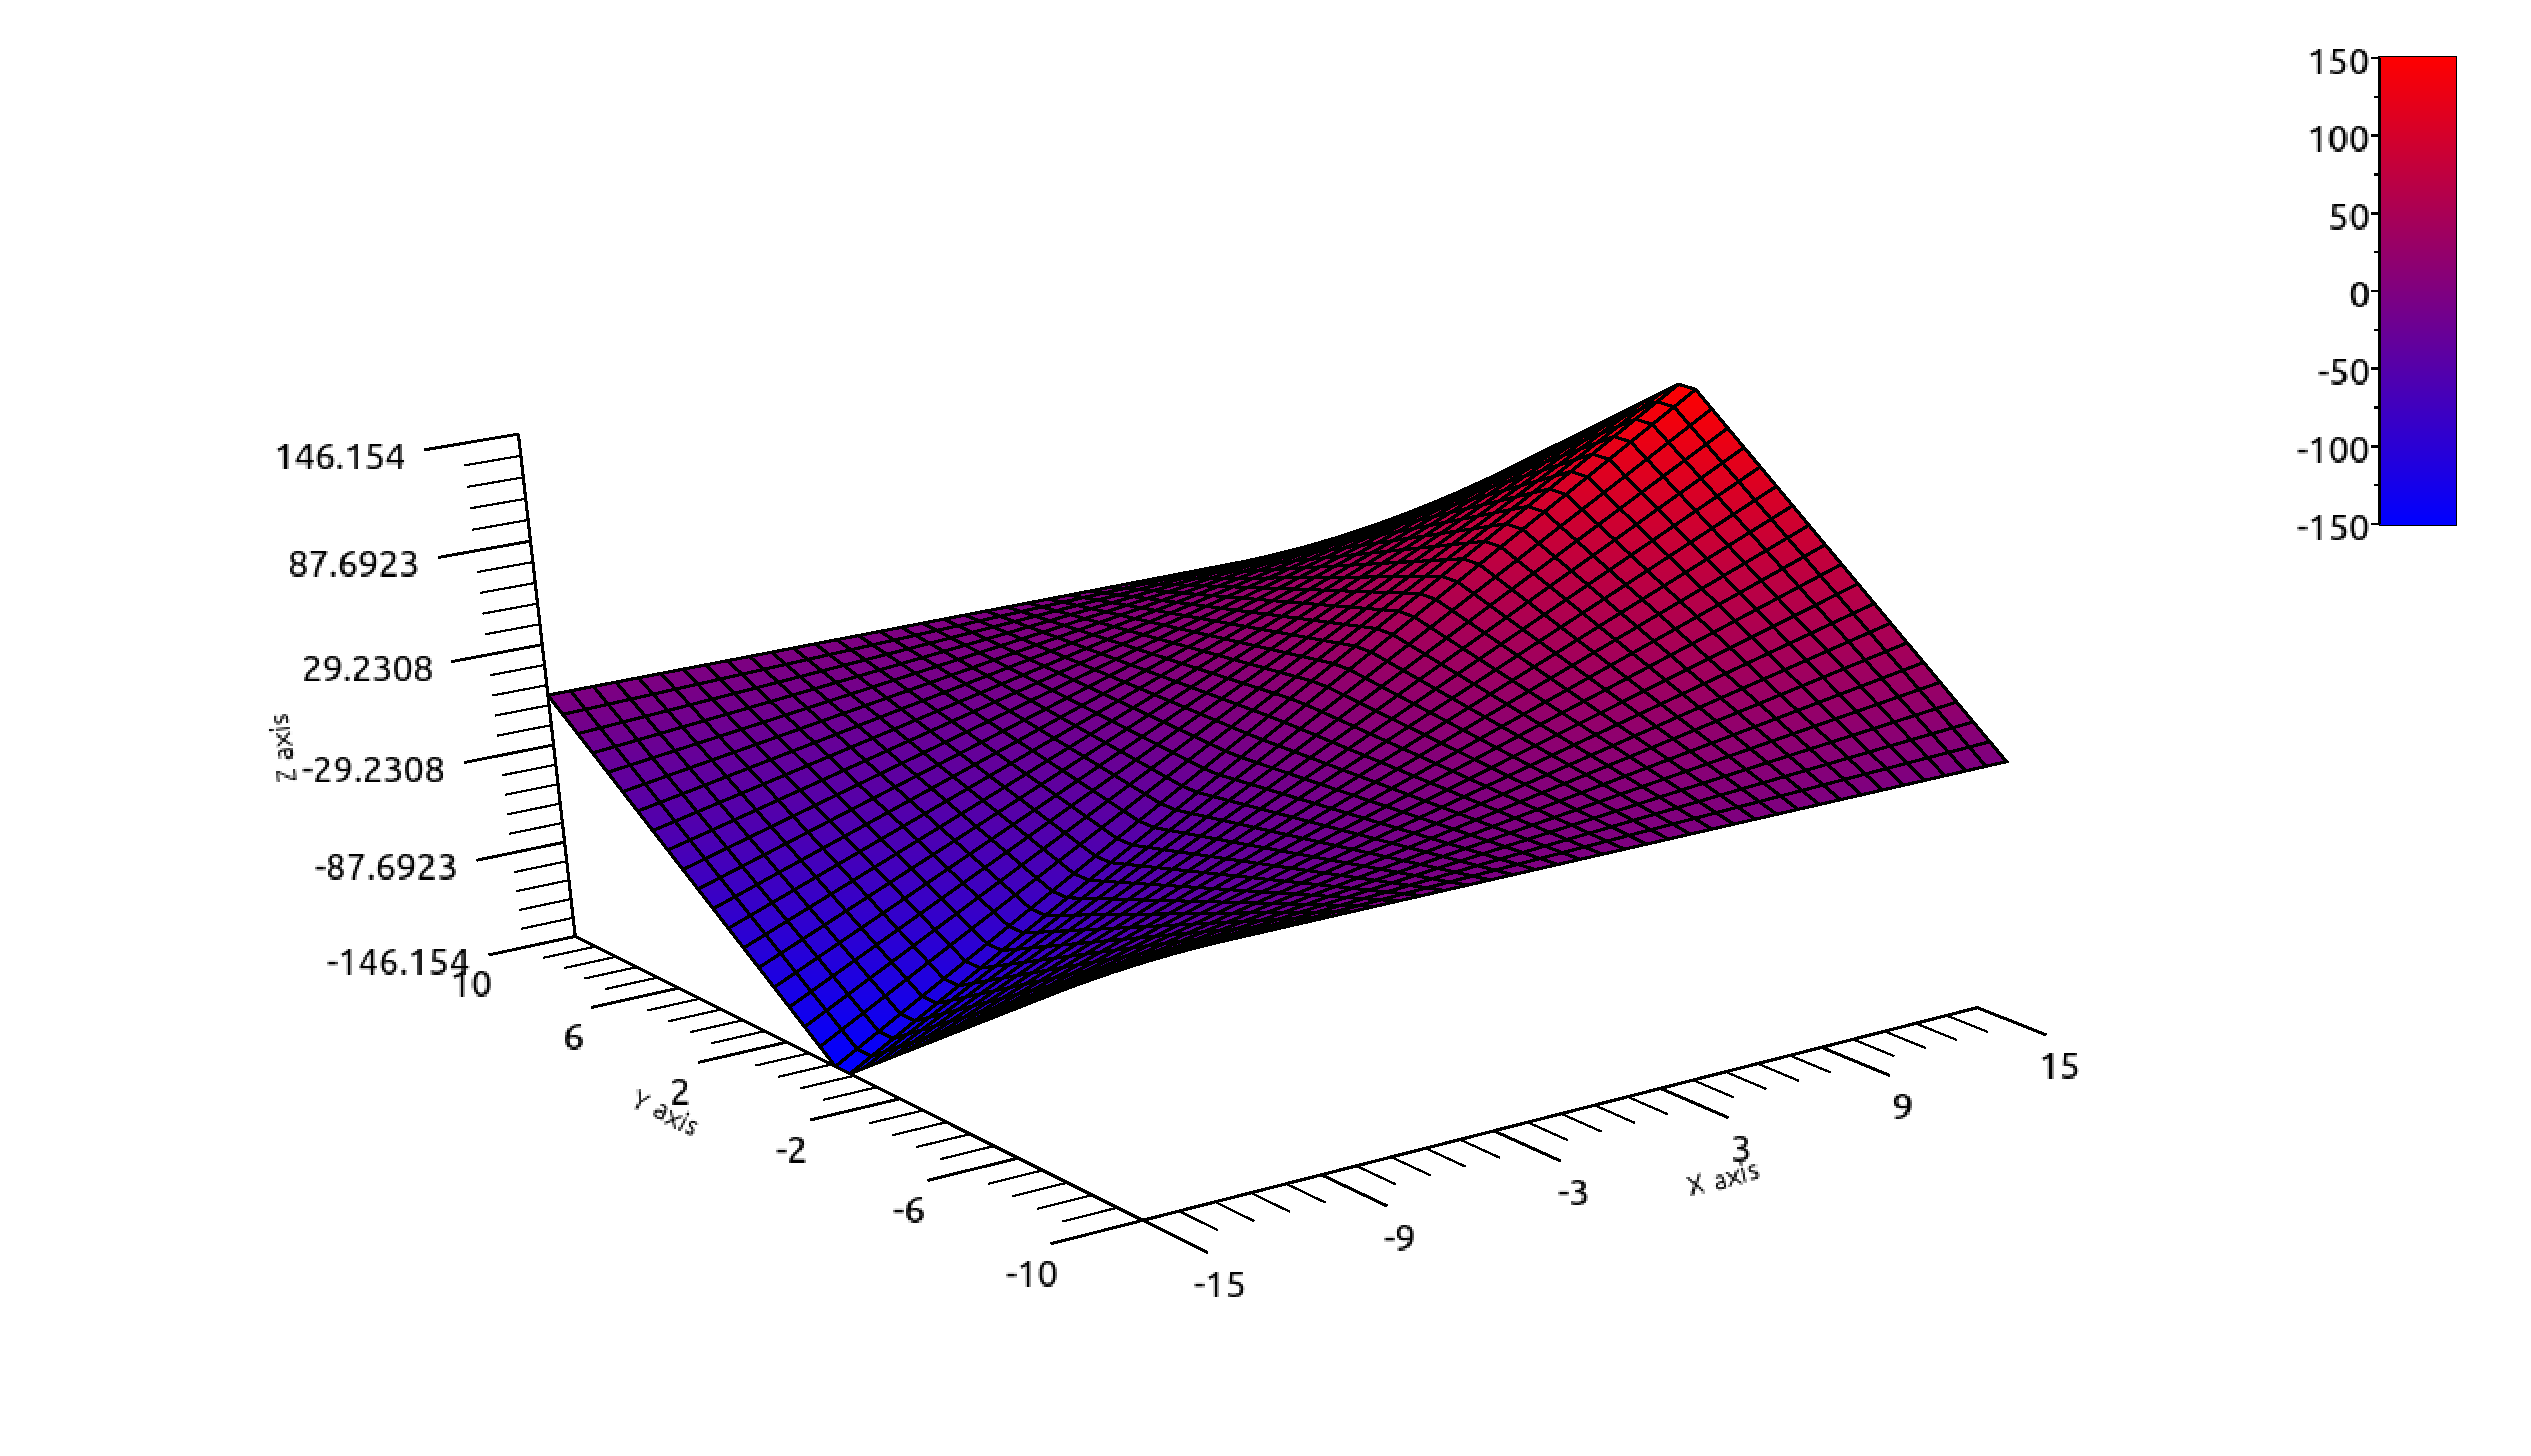
\includegraphics[width=\textwidth]{Chapter4/figures/Graph1.pdf}
\end{figure}
\end{frame}





\subsection*{Active Players Coordination}
\begin{frame}
 	 \frametitle{Determination of Active Positions}
 	 
 	 \begin{itemize}[<+->]
 	 \item Dynamic production of active positions.	 	 
 	 \begin{figure}[t!]
\centering
  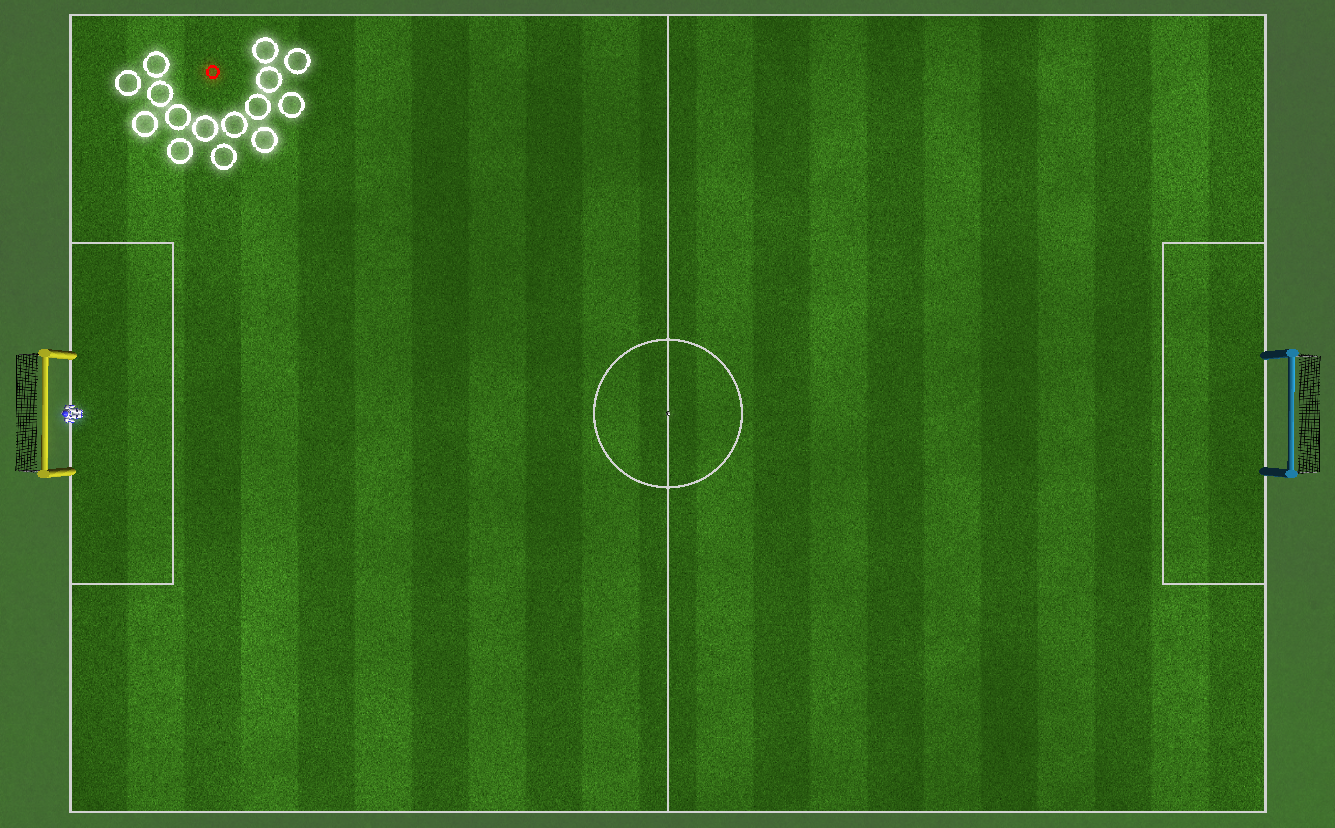
\includegraphics[height=2.5cm, width=3cm, clip, trim=0cm 10cm 20cm 0cm]{Chapter4/figures/ActiveBefore(-8,6).png} \quad	
  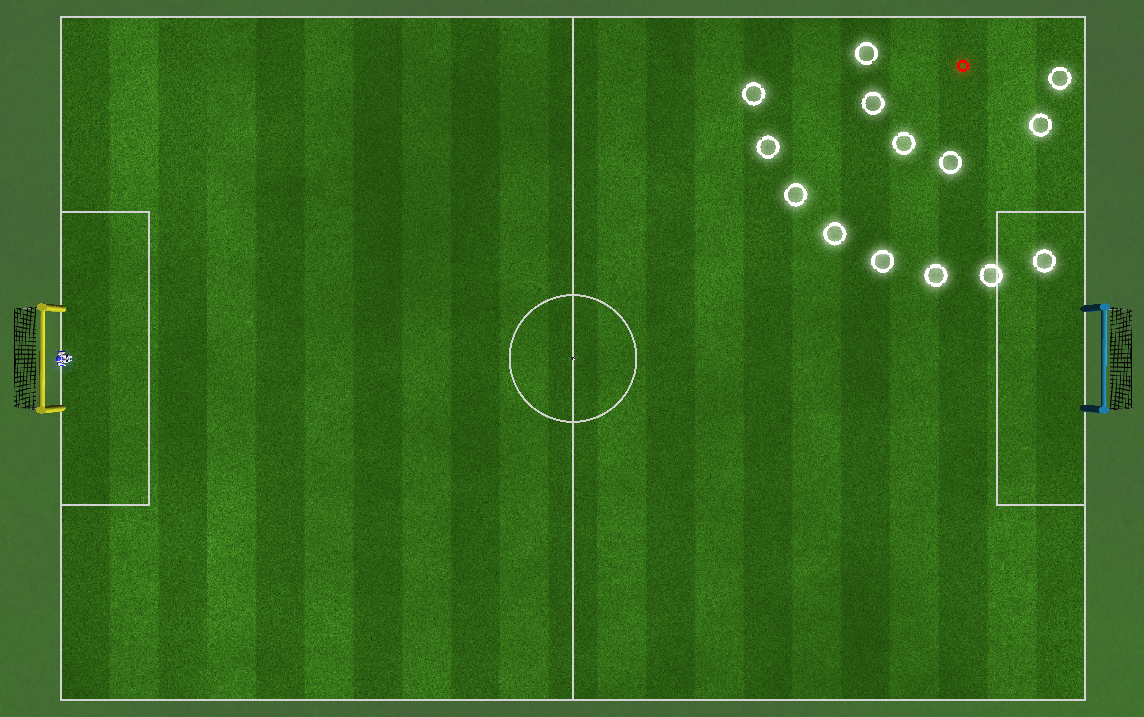
\includegraphics[height=2.5cm, width=3cm, clip, trim=20cm 10cm 0cm 0cm]{Chapter4/figures/ActiveBefore(8,6).png}
\end{figure}

\item Positions elimination making use of their utility field value.
\item Max number of 9 positions.
\begin{figure}[t!]
\centering
  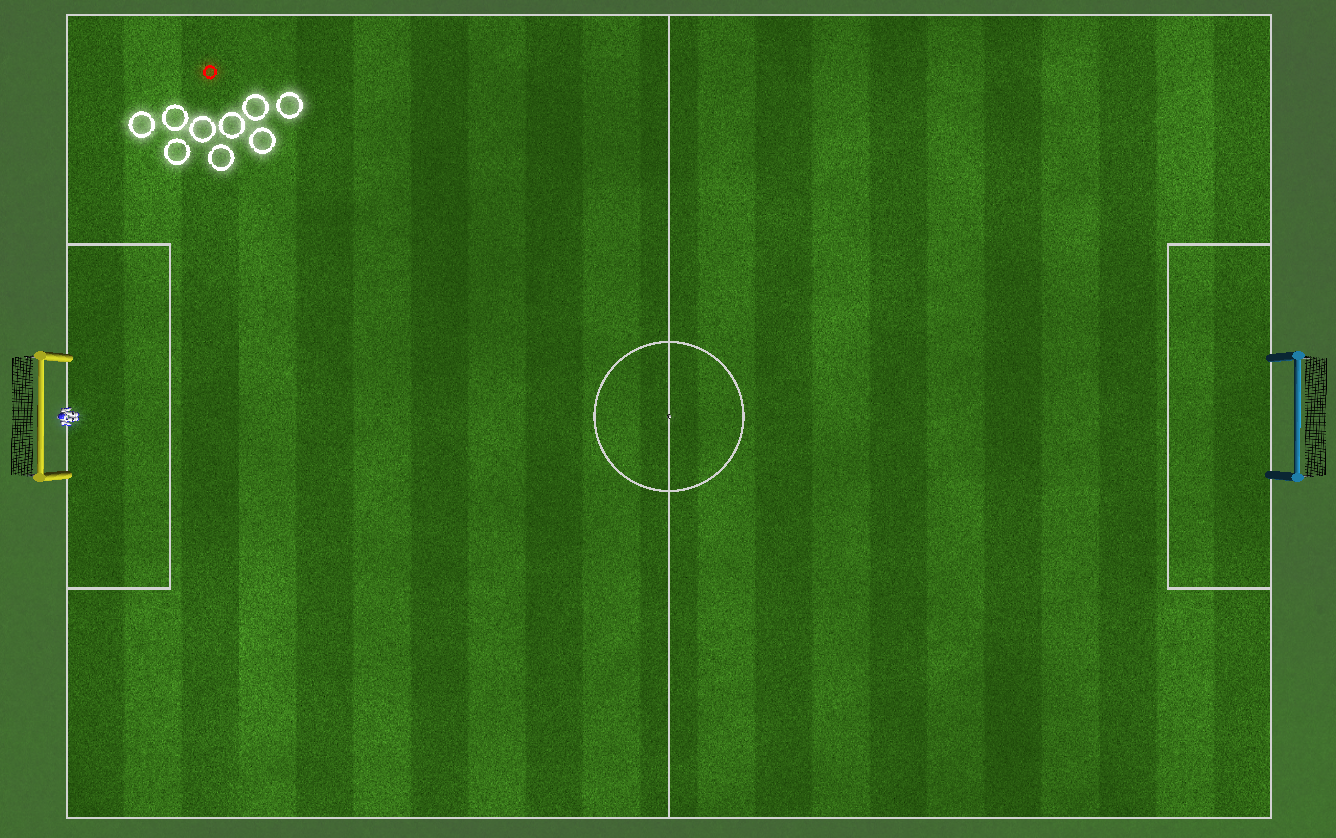
\includegraphics[height=2.5cm, width=3cm, clip, trim=0cm 10cm 20cm 0cm]{Chapter4/figures/ActiveAfter(-8,6).png} \quad	
  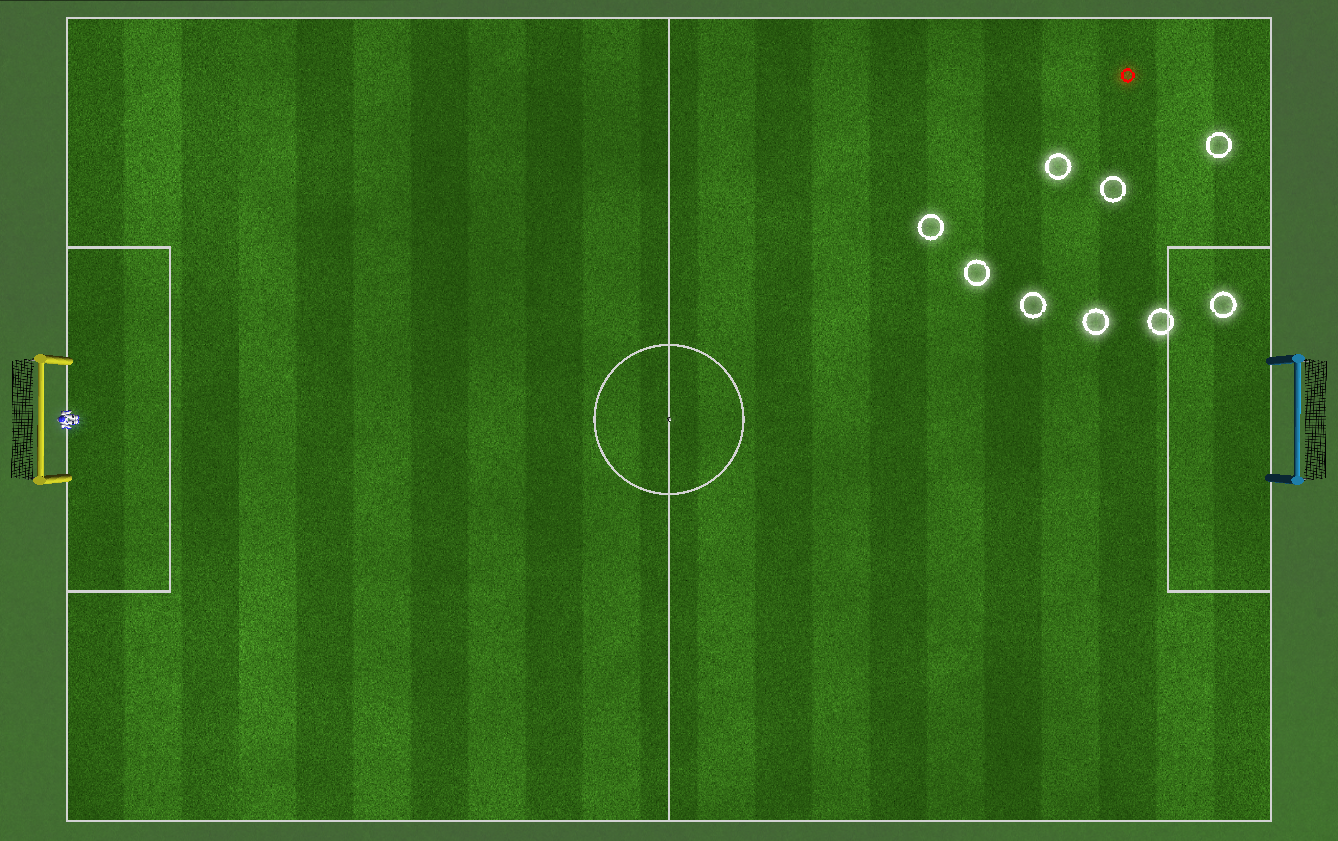
\includegraphics[height=2.5cm, width=3cm, clip, trim=20cm 10cm 0cm 0cm]{Chapter4/figures/ActiveAfter(8,6).png}
\end{figure}
 	 
 	 
 	 \end{itemize}
\end{frame}




\begin{frame}
 	 \frametitle{Active Players Coordination}
 	 \begin{itemize}[<+->]
 	 \item On Ball player.
 	 \item Agent closest to the ball.
 	 \item Angle from goal is also taken into consideration.
 	 \item Set of $\leq$ 9 positions.
 	 \item Set of $\leq$ 2 agents.
 	 \item Exhaustive algorithm.
 	 \item Every combination of mappings is checked.
  	 \item Cost function to determine which of them is optimal.	 
 	 \end{itemize}
 	 
\end{frame}


\begin{frame}
 	 \frametitle{Active Coordination Evaluation Function}
The evaluation function scores each possible mapping using the following features defined for each agent $i$: 
\begin{enumerate}
\item \textbf{Distance} $C_{d,i}$
\item \textbf{Potential Collisions} $C_{c,i}$
\item \textbf{Field Utility} $C_{u,i}$
\item \textbf{Close Targets} $C_{t,i}$
\item \textbf{Horizontal Stretch} $C_{h,i}$
\end{enumerate}
\begin{align*}
ActiveCost(ActiveMapping) &= \sum_{i=1}^3 w_dC_{d,i}+w_cC_{c,i}-w_uC_{u,i}-w_tC_{t,i}-w_hC_{h,i}
\end{align*}
where $(w_d,w_c,w_u,w_t,w_h)$ are the weights of the features, currently set at $(1,1,1/7,1,1)$.
\end{frame}
  
  \subsection*{Team Formation}
  \begin{frame}
 	 \frametitle{Generation of Team Formation}
  Serves to set up the role assignment function and the coordination of the support subset.
  \begin{itemize}
 	 \item 9 Players Version.
 	 \item 11 Players Version. 	 
  \end{itemize}
  \begin{figure}[t!]
\centering
  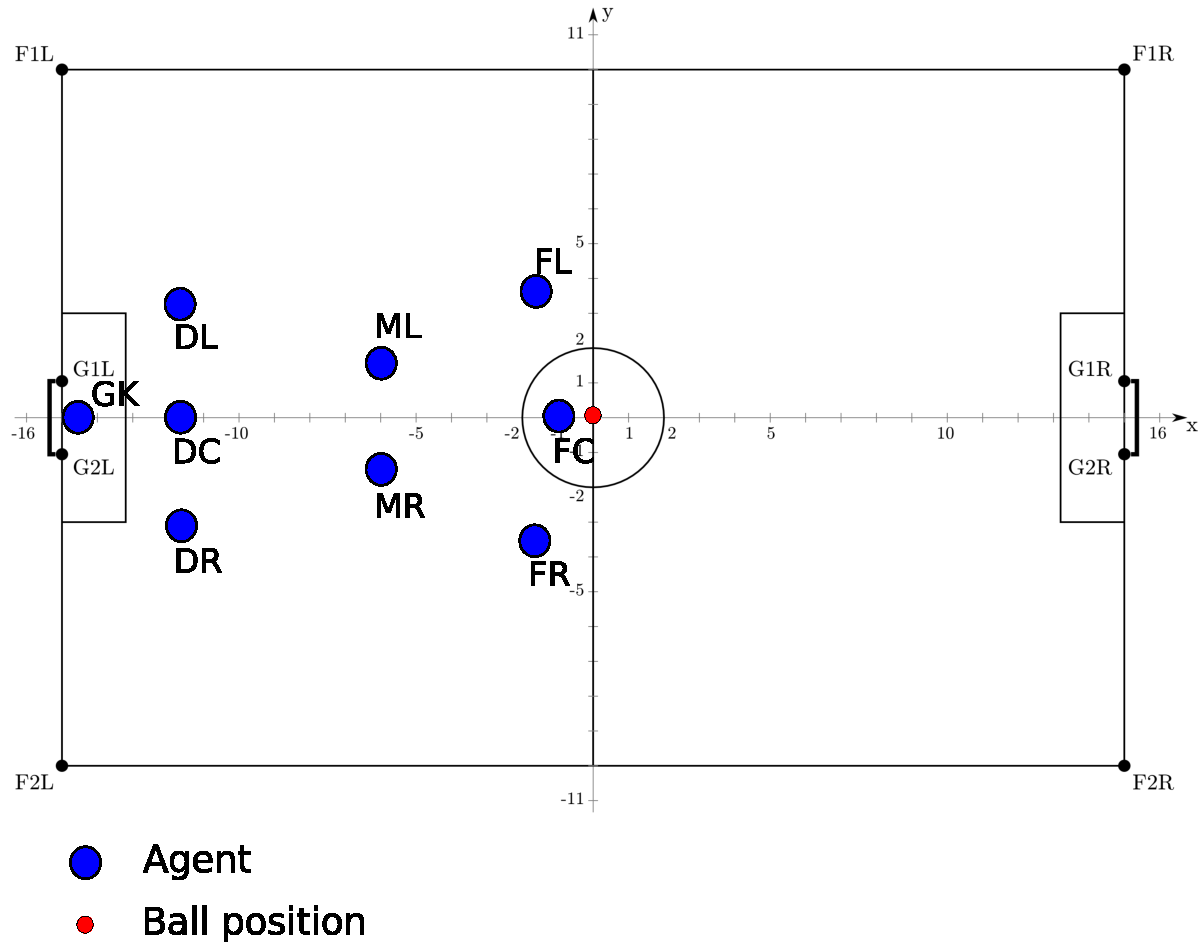
\includegraphics[width=0.33\textwidth]{Chapter4/figures/Formation9_0.pdf}\quad
  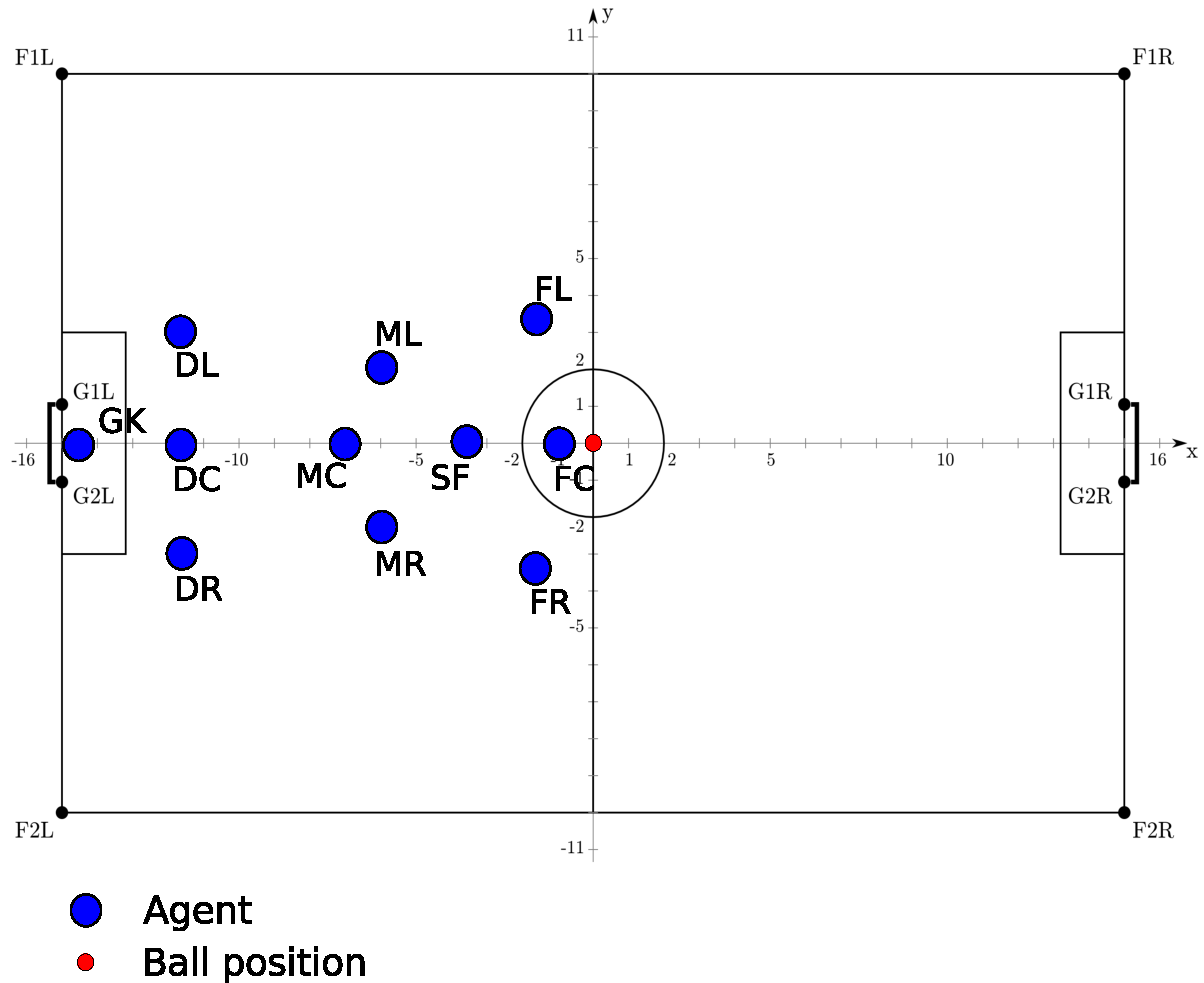
\includegraphics[width=0.37\textwidth]{Chapter4/figures/Formation11_0.pdf}
\end{figure}
  \end{frame}
  
  \begin{frame}
 	 \frametitle{Team Formation Examples}
 	 \begin{figure}[t!]
\centering
  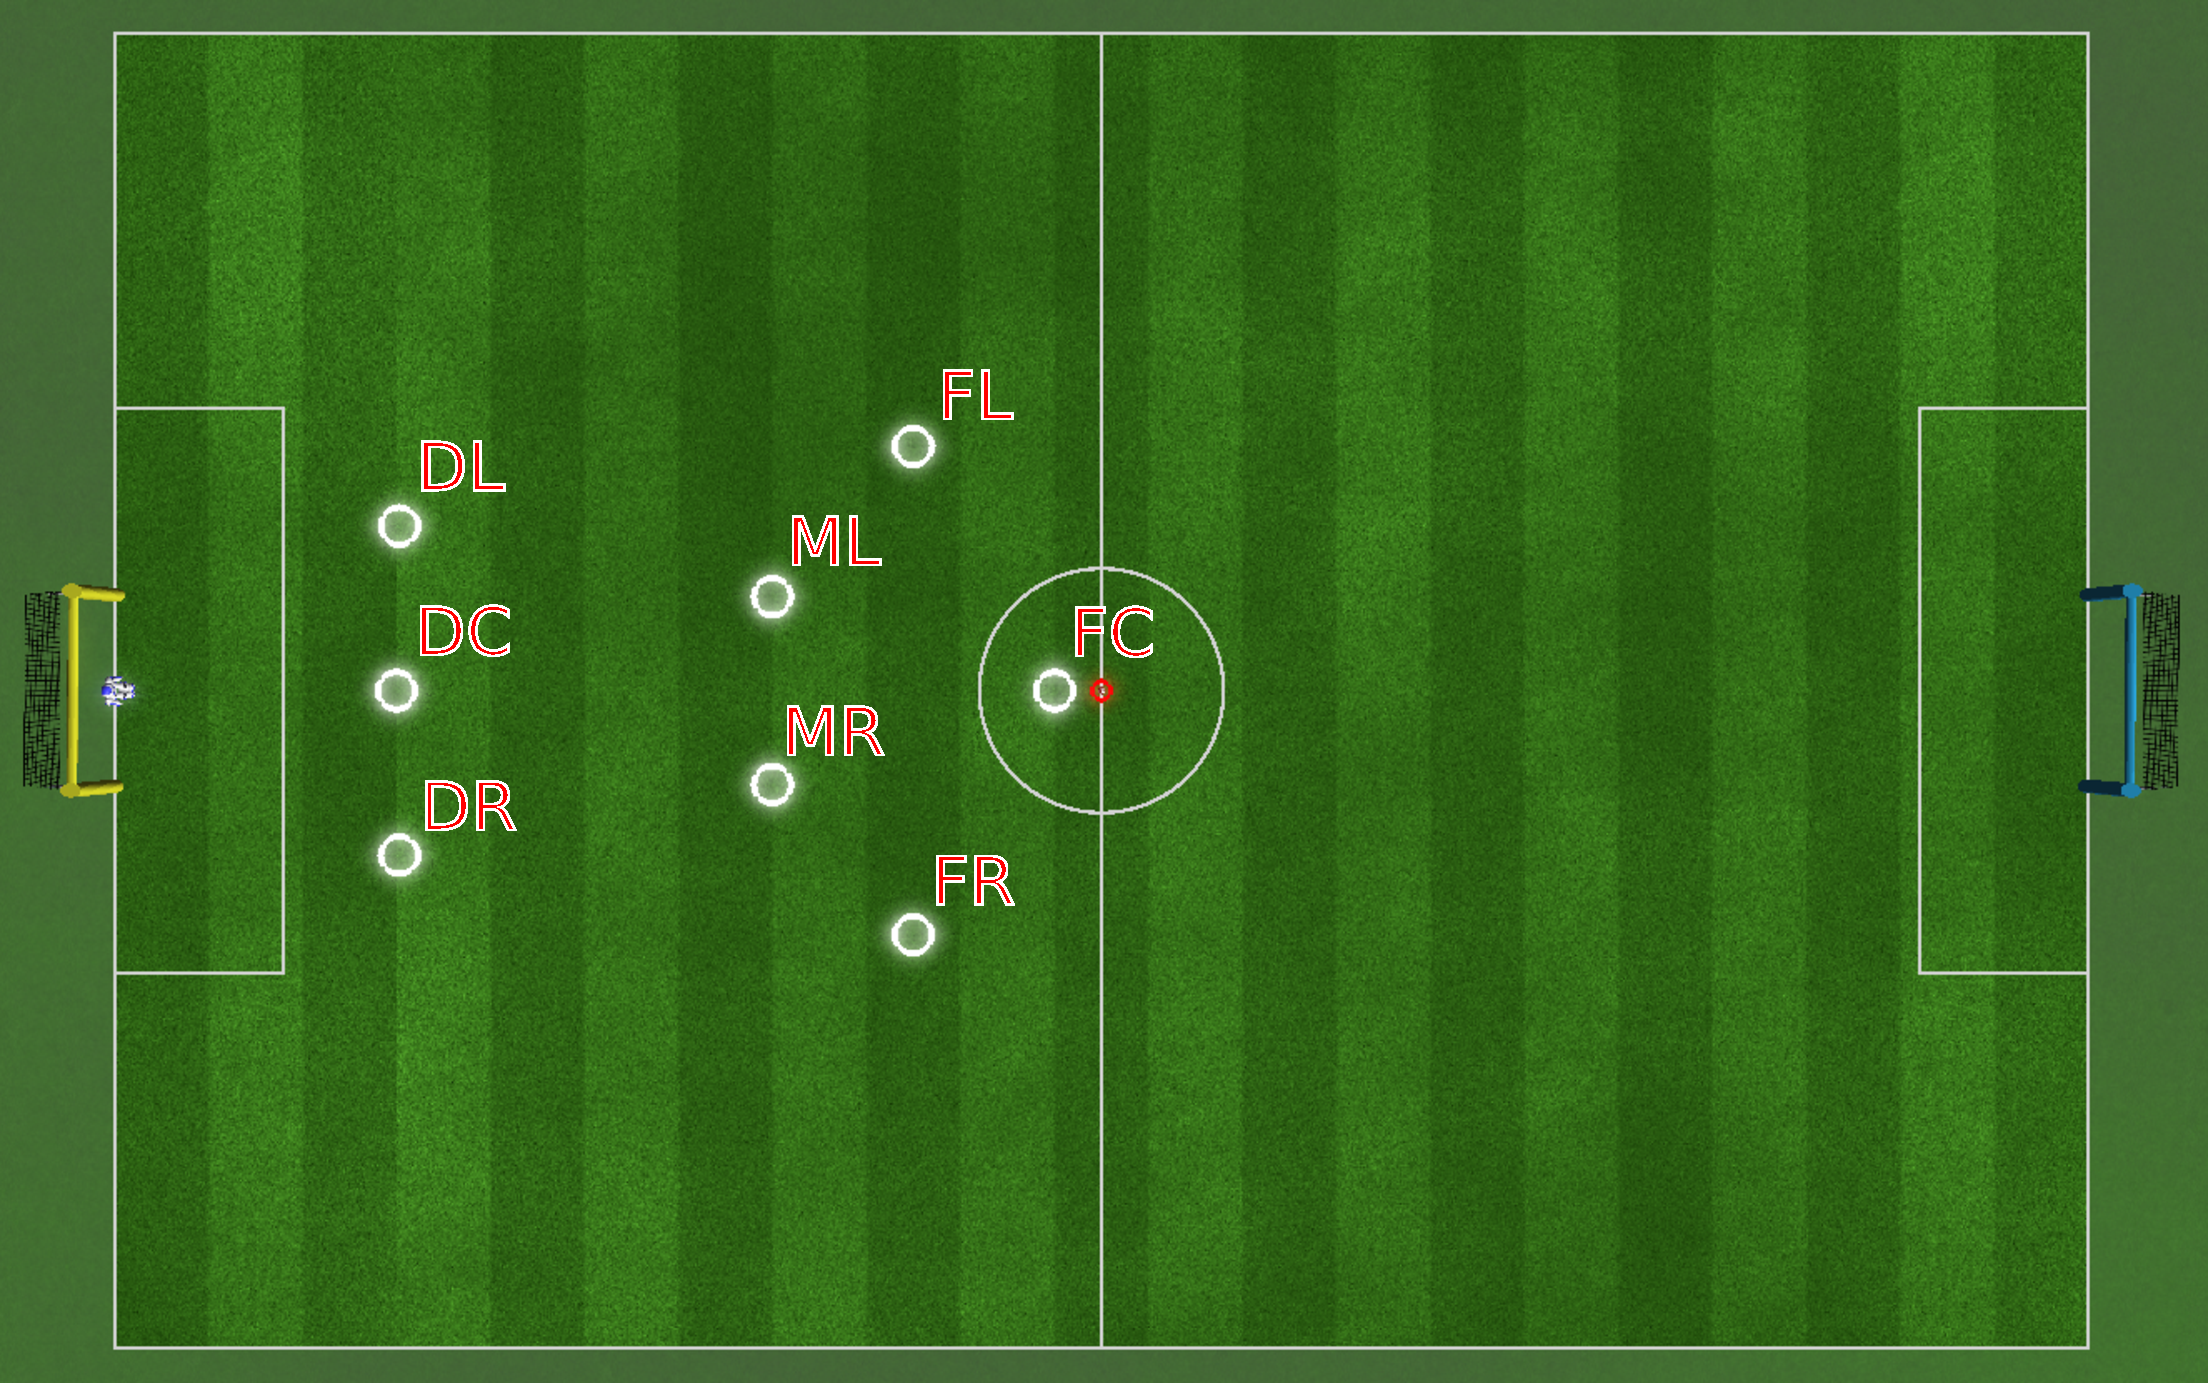
\includegraphics[height=0.36\textheight]{Chapter4/figures/Formation(0,0).pdf}\	
  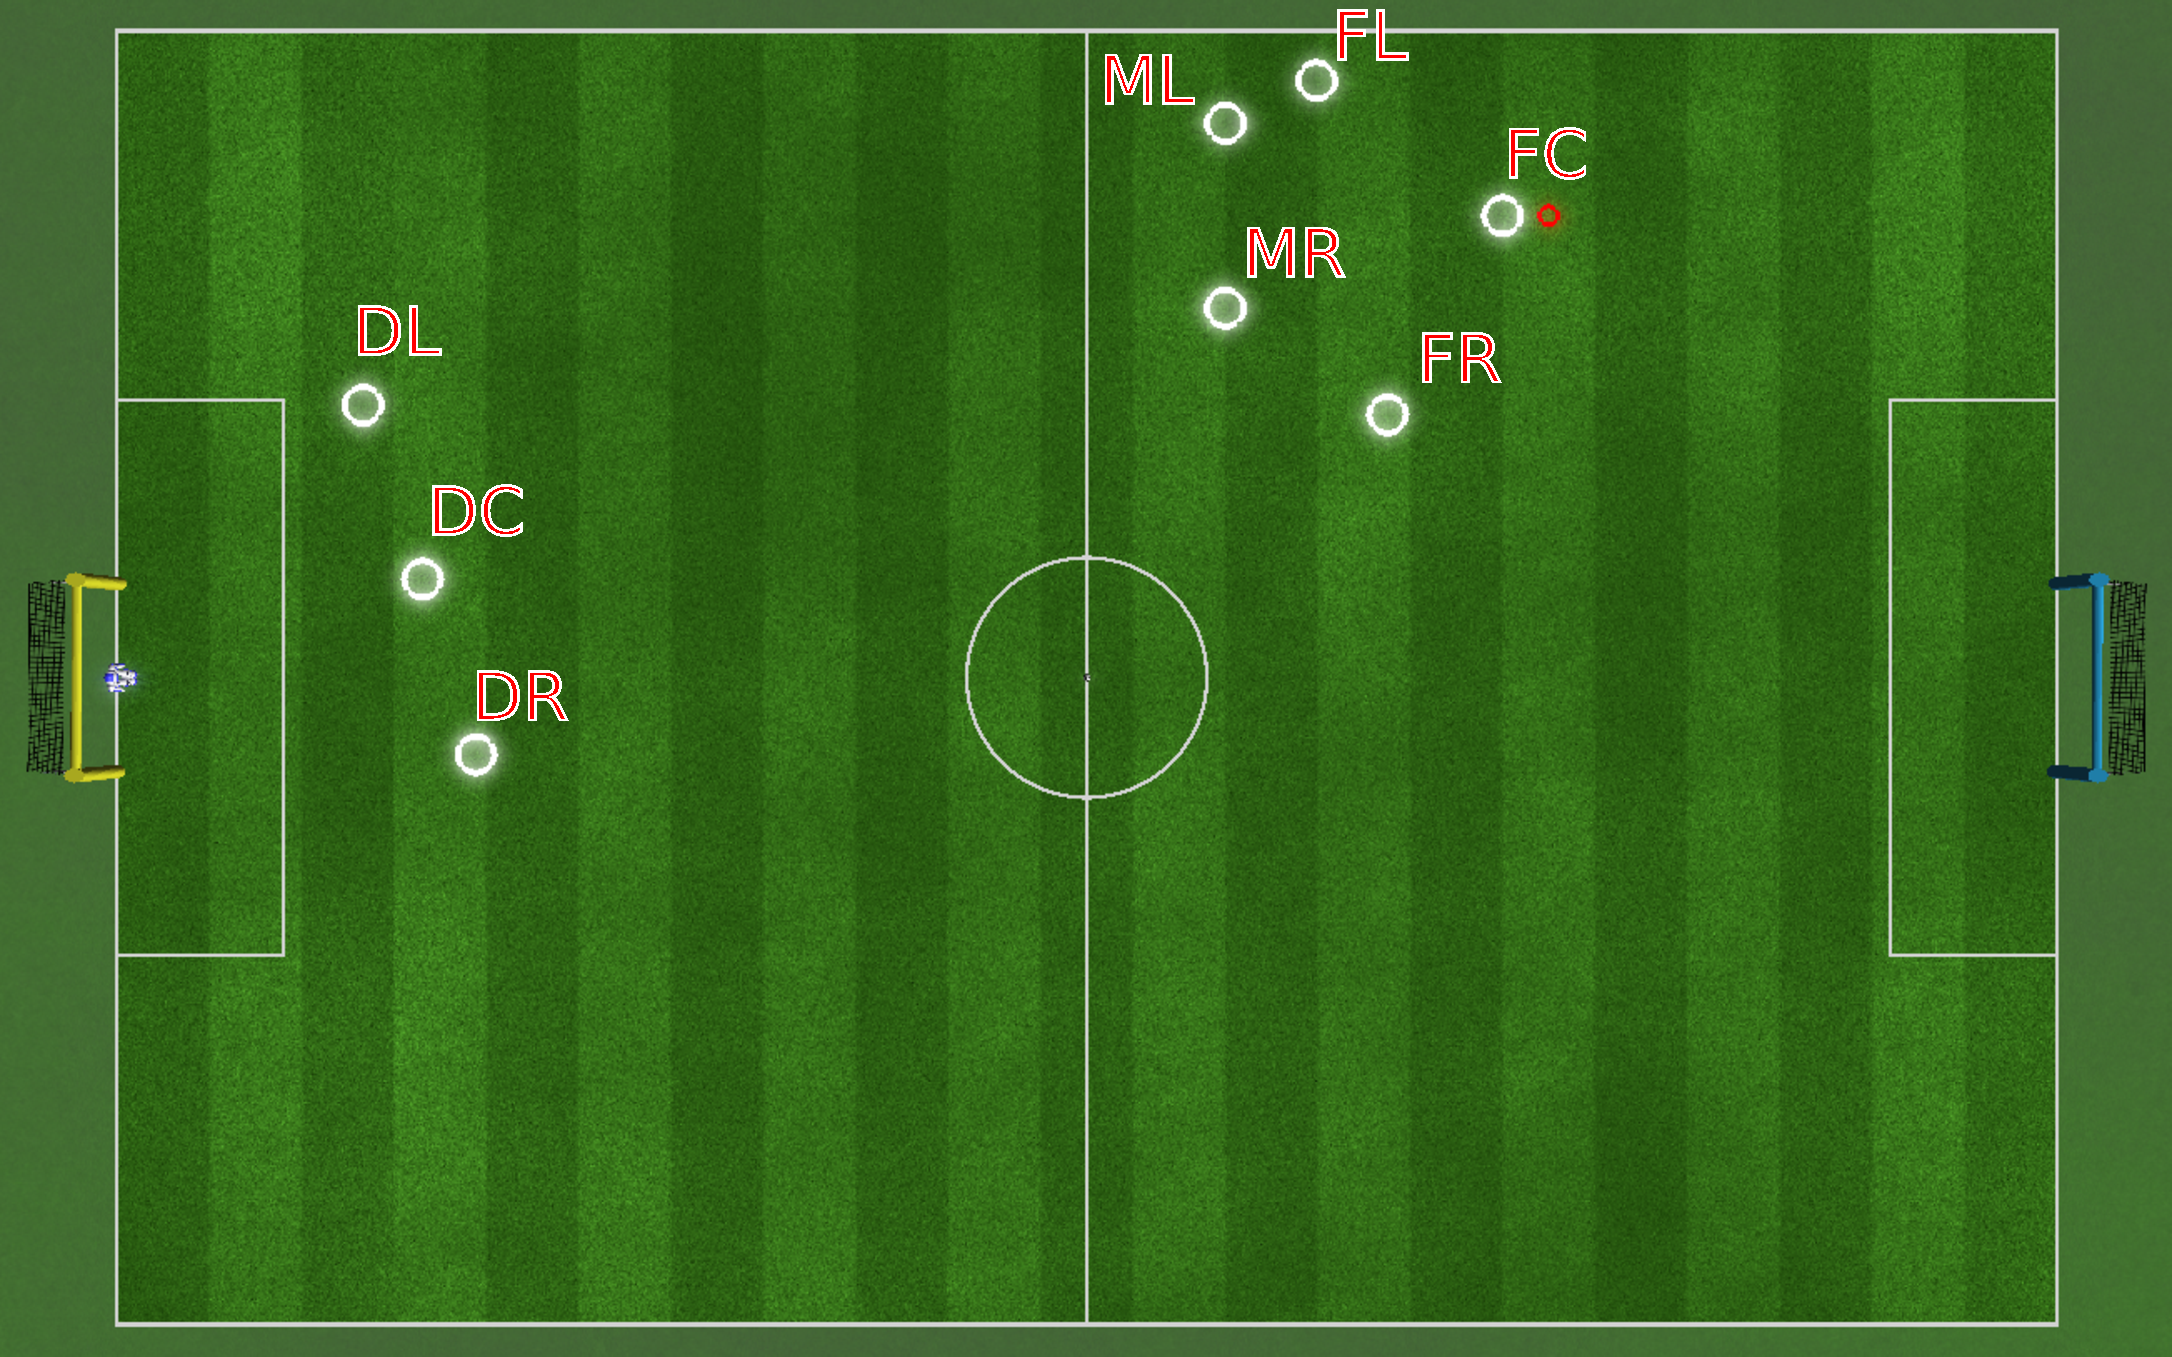
\includegraphics[height=0.36\textheight]{Chapter4/figures/Formation(5,5).pdf}\\ \vspace{0.1cm}
  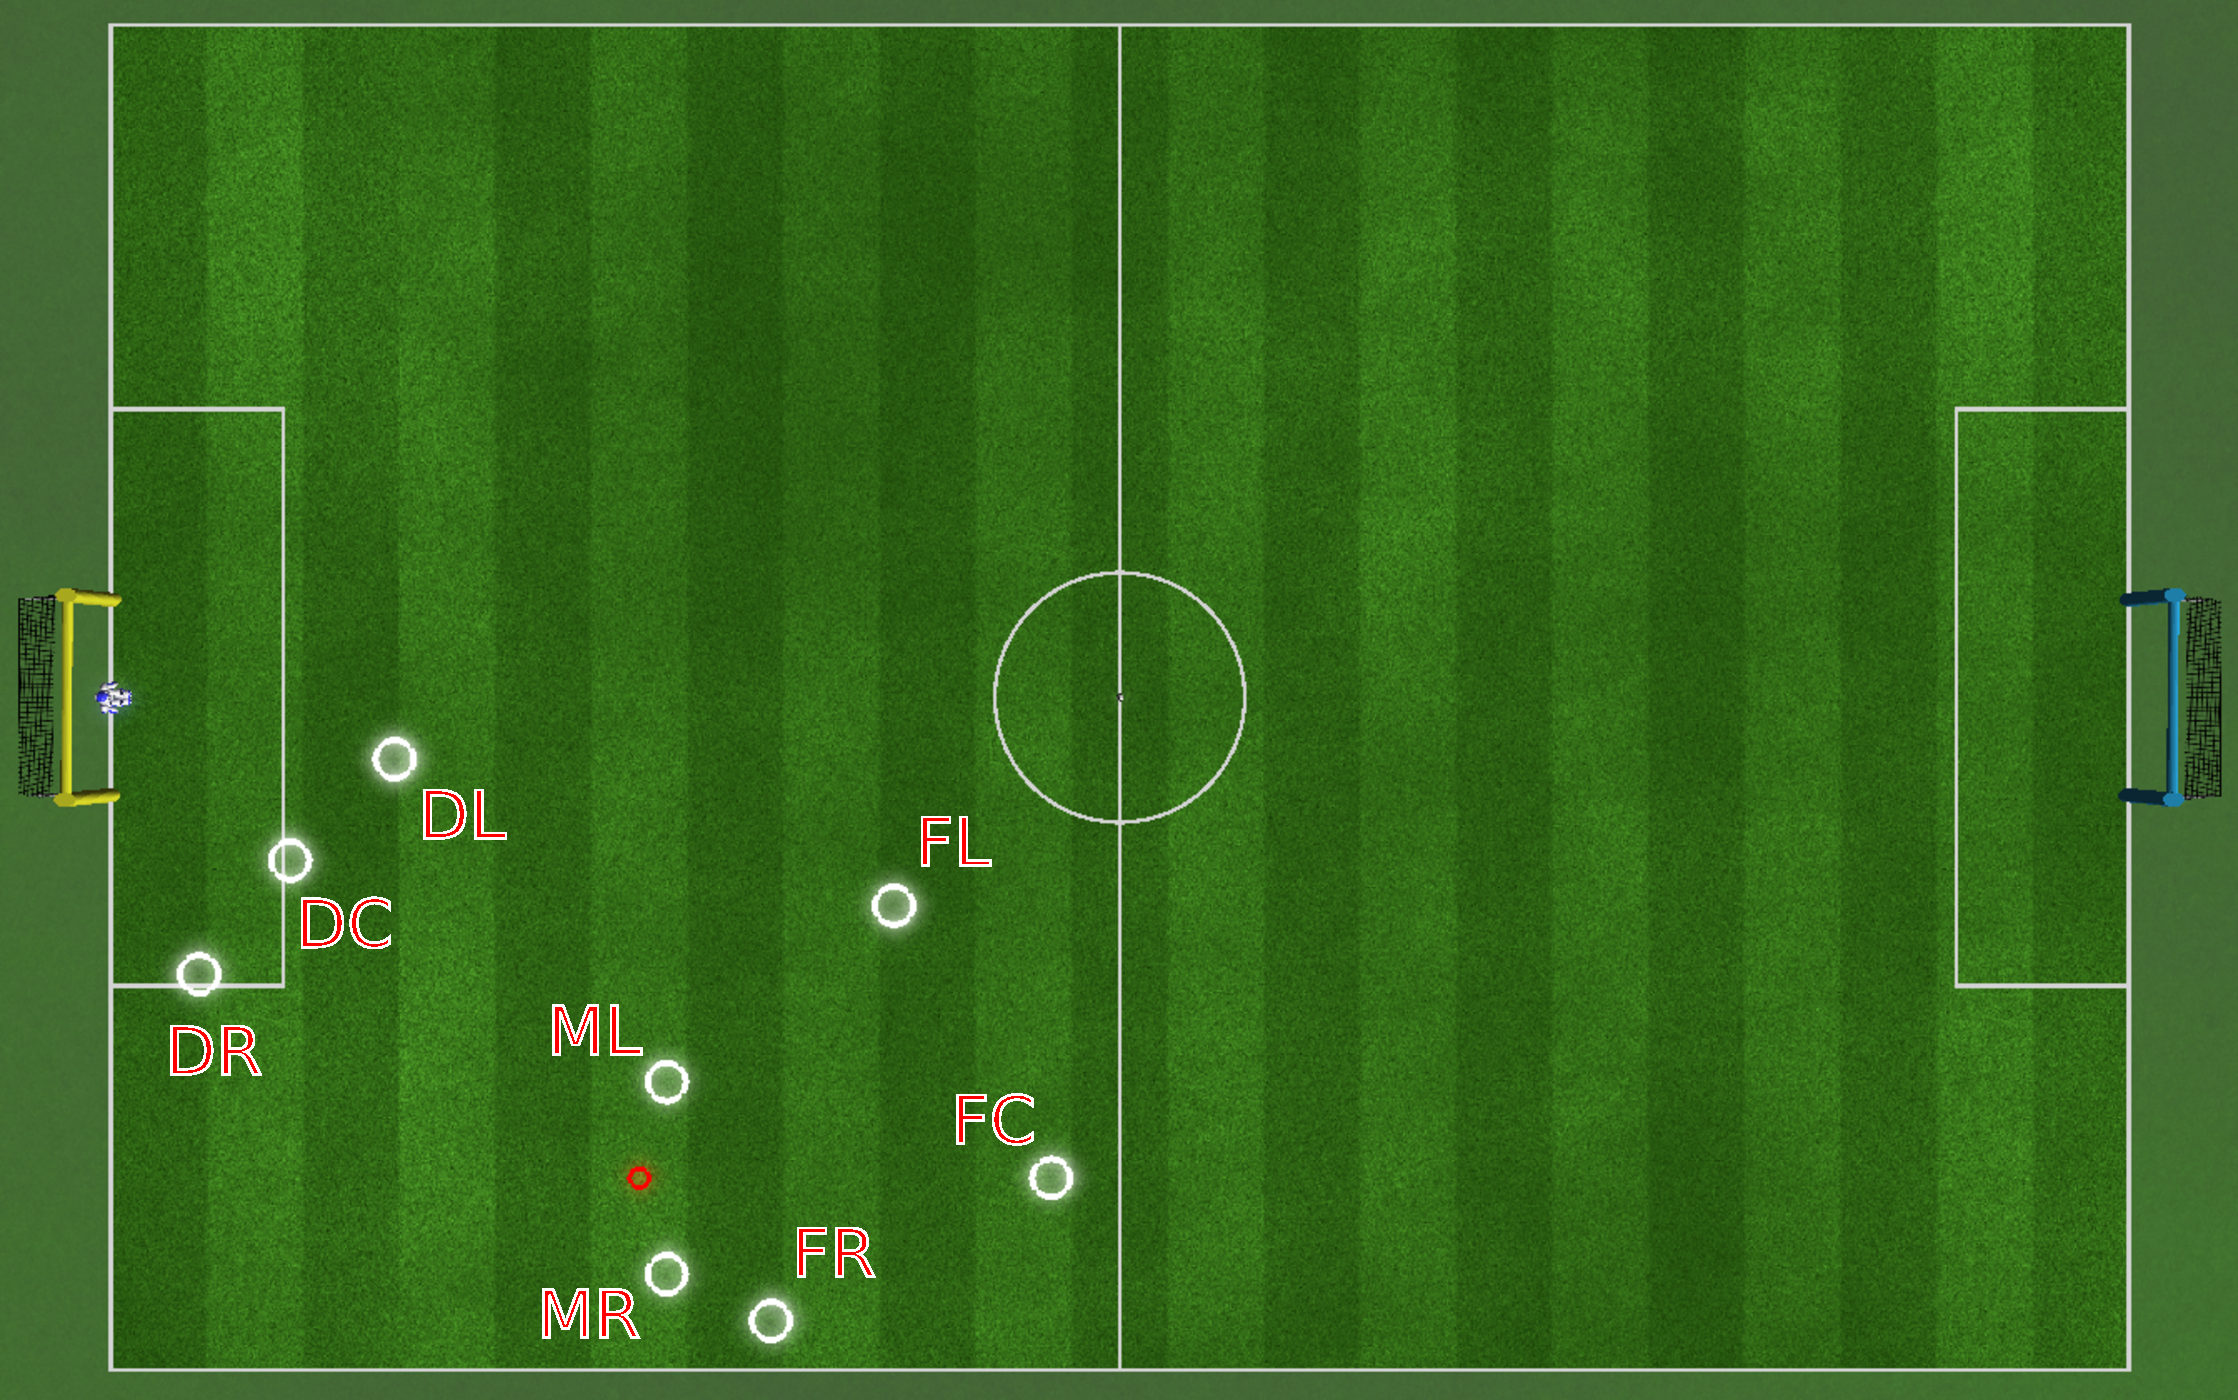
\includegraphics[height=0.36\textheight]{Chapter4/figures/Formation(-5,-5).pdf}
\end{figure}
  \end{frame}
  
  
\subsection*{Team Roles Assignment}
  \begin{frame}
 	 \frametitle{Team Roles Assignment}
 	 \begin{itemize}[<+->]
 	 \item Assigns roles to all agents.
 	 \item Roles close to ball, active players.
 	 \item Remaining roles will be assigned to support players.
 	 \item Inactive agents.
 	 \item Same number of roles will be discarded.
 	 \end{itemize}

 \end{frame}
  
  \begin{frame}
 	 \frametitle{Team Roles Assignment Example 1}
 	 \begin{figure}[t!]
\centering
  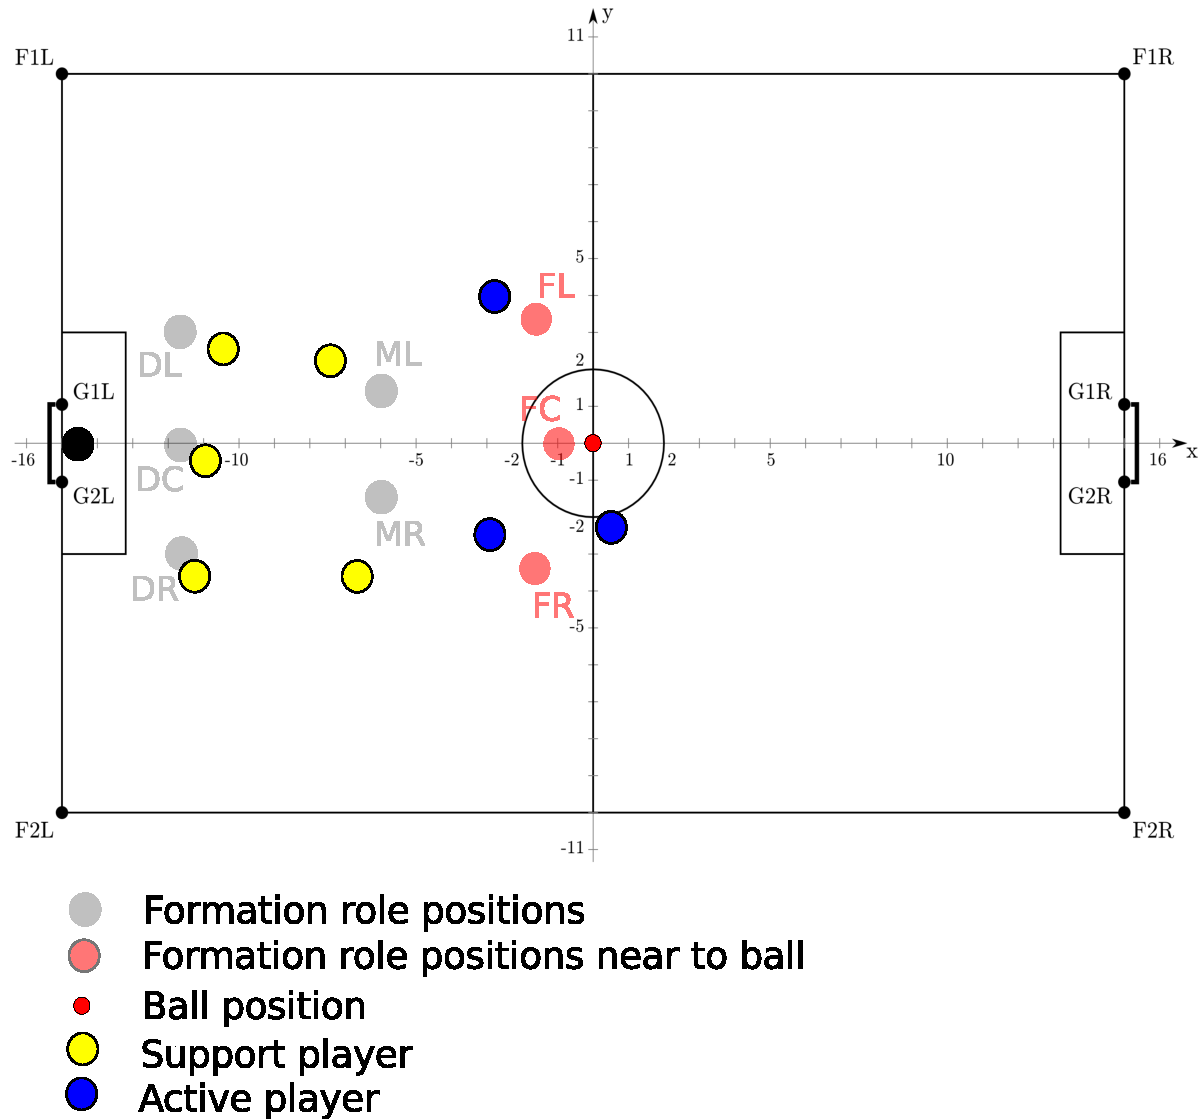
\includegraphics[width=0.6\textwidth]{Chapter4/figures/RoleAss.pdf}
\end{figure}
  \end{frame}
  
  \begin{frame}
 	 \frametitle{Team Roles Assignment Example 2}
 	 \begin{figure}[t!]
\centering
  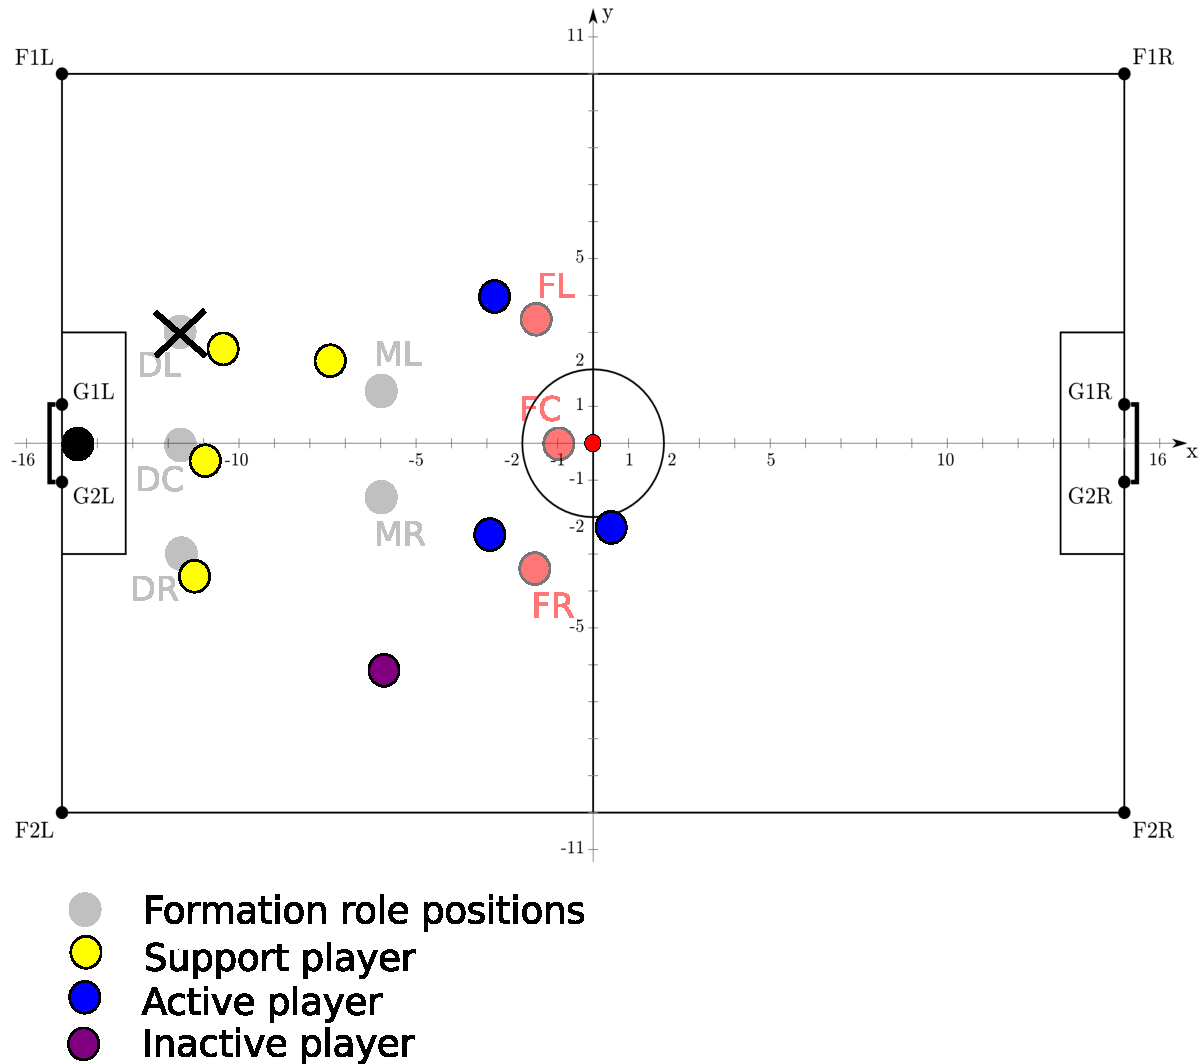
\includegraphics[width=0.6\textwidth]{Chapter4/figures/SupportPos.pdf}
\end{figure}
  \end{frame}
  
  
	\subsection*{Support Players Coordination} 
	\begin{frame}
 	 \frametitle{Team Roles Assignment Example 1}
 	 \begin{itemize}[<+->]
 	 \item Same number of positions, agents.
 	 \item Computationally expensive problem.
 	 \item The exhaustive algorithm, in a worst case scenario, would have to examine between 40320 and 3628800 possible mappings.
 	 \item The exhaustive algorithm can work satisfactorily on support subsets of size up to 6 (720 possible mappings).
 	 \end{itemize}
  \end{frame}
  
  \begin{frame}
 	 \frametitle{Dynamic Algorithm}
 	 \begin{itemize}[<+->]
 	 \item Given the difficulties of applying the exhaustive algorithm.
 	 \item A method proposed by the UT Austin Villa team.
 	 \item Able to compute an approximately optimal solution.
 	 
 	   	\begin{table}[t!]
\begin{center}
\begin{tiny}
\begin{tabular}{ | c | c | c | }
    \hline
    $\lbrace P_{1} \rbrace$   & $\lbrace P_{1},P_{2} \rbrace$ 	& $\lbrace P_{1},P_{2},P_{3} \rbrace$\\ \hline
    $\lbrace A_{1} \leftarrow P_{1}\rbrace$ & $\lbrace A_{1} \leftarrow P_{2}\rbrace \cup \arg\min(\lbrace A_{2} \rbrace \leftarrow \lbrace P_{1}\rbrace)$	 	& $\lbrace A_{1} \leftarrow P_{3}\rbrace \cup \arg\min(\lbrace A_{2},A_{3} \rbrace \leftarrow \lbrace P_{1},P_{2} \rbrace)$  \\ 
    $\lbrace A_{2} \leftarrow P_{1}\rbrace$ & $\lbrace A_{1} \leftarrow P_{2}\rbrace \cup\arg\min(\lbrace A_{3}  \rbrace \leftarrow \lbrace  P_{1} \rbrace)$	 	& $\lbrace A_{2} \leftarrow P_{3}\rbrace \cup\arg\min(\lbrace A_{1},A_{3} \rbrace \leftarrow \lbrace P_{1},P_{2} \rbrace)$  \\ 
$\lbrace A_{3} \leftarrow P_{1}\rbrace$  & $\lbrace A_{2} \leftarrow P_{2}\rbrace \cup\arg\min(\lbrace A_{1}  \rbrace \leftarrow \lbrace  P_{1} \rbrace)$ 		& $\lbrace A_{3} \leftarrow P_{3}\rbrace \cup\arg\min(\lbrace A_{1},A_{2} \rbrace \leftarrow \lbrace P_{1},P_{2} \rbrace)$  \\ 
       						  & $\lbrace A_{2} \leftarrow P_{2}\rbrace \cup\arg\min(\lbrace A_{3}  \rbrace \leftarrow \lbrace  P_{1} \rbrace)$ 		&   \\ 
       						  & $\lbrace A_{3} \leftarrow P_{2}\rbrace \cup\arg\min(\lbrace A_{1}  \rbrace \leftarrow \lbrace  P_{1} \rbrace)$ 		&   \\ 
    						  & $\lbrace A_{3} \leftarrow P_{2}\rbrace \cup\arg\min(\lbrace A_{2}  \rbrace \leftarrow \lbrace P_{1} \rbrace)$		&   \\
    \hline
    \end{tabular}      
\end{tiny}
\end{center}	
\end{table}
  	\end{itemize}
  \end{frame}
  
  
  \begin{frame}
 	 \frametitle{Dynamic Algorithm Complexity}
 	 \begin{itemize}[<+->]
 	 \item In $k$th iteration of the algorithm, each agent will be assigned to the $P_{k}$ position.
 	 \item The previous $k-1$ positions will be assigned to the other $n-1$ agents.
 	 \item Result in a total of $ {{n-1}\choose{k-1}} $ mappings to be evaluated in each iteration for each agent.
 	 \[
n \sum_{k=1}^n {{n-1}\choose{k-1}} = n \sum_{k=0}^{n-1}{{n-1}\choose{k}} = n 2^{n-1}
\]

	\item This represents a reduction to $1024$ and $5120$ mappings for $8$ and $10$ agents/positions respectively compared to $40320$ and $3628800$ mappings of the exhaustive algorithm.
 	 \end{itemize}
  \end{frame}
  
  \subsection*{Goalkeeper Behavior}
  \begin{frame}
 	 \frametitle{Dynamic Algorithm Complexity}
 	 \begin{itemize}[<+->]
  \item Only agent in our team who ``runs'' his own behavior.
  \item His behavior depends on a finite state machine.
  
  \begin{figure}[t!]
\begin{center}
\begin{tikzpicture}[->,>=stealth',shorten >=1pt,node distance=3.5cm,auto]
\node[state,initial] 		(q_1) {\textbf{Localize}};
\node[state]  			    (q_2) [right of = q_1] {\textbf{Guard}};
\node[state] 				(q_3) [right of = q_2] {\textbf{Libero}};
\draw[->] (q_1) edge [bend left=15] node {in position} (q_2);
\draw[->] (q_2) edge [bend left=30] node {ball in goal area} (q_3);
\draw[->] (q_2) edge [bend left=15] node {after fall} (q_1);
\draw[->] (q_3) edge [bend left=40] node {ball cleared} (q_1);
\end{tikzpicture}
\end{center}
\end{figure} 

  \end{itemize}
  \end{frame}
  
  
  
\begin{frame}
 	 \frametitle{``Guard'' State}
 	 \begin{figure}[t!]
\centering
  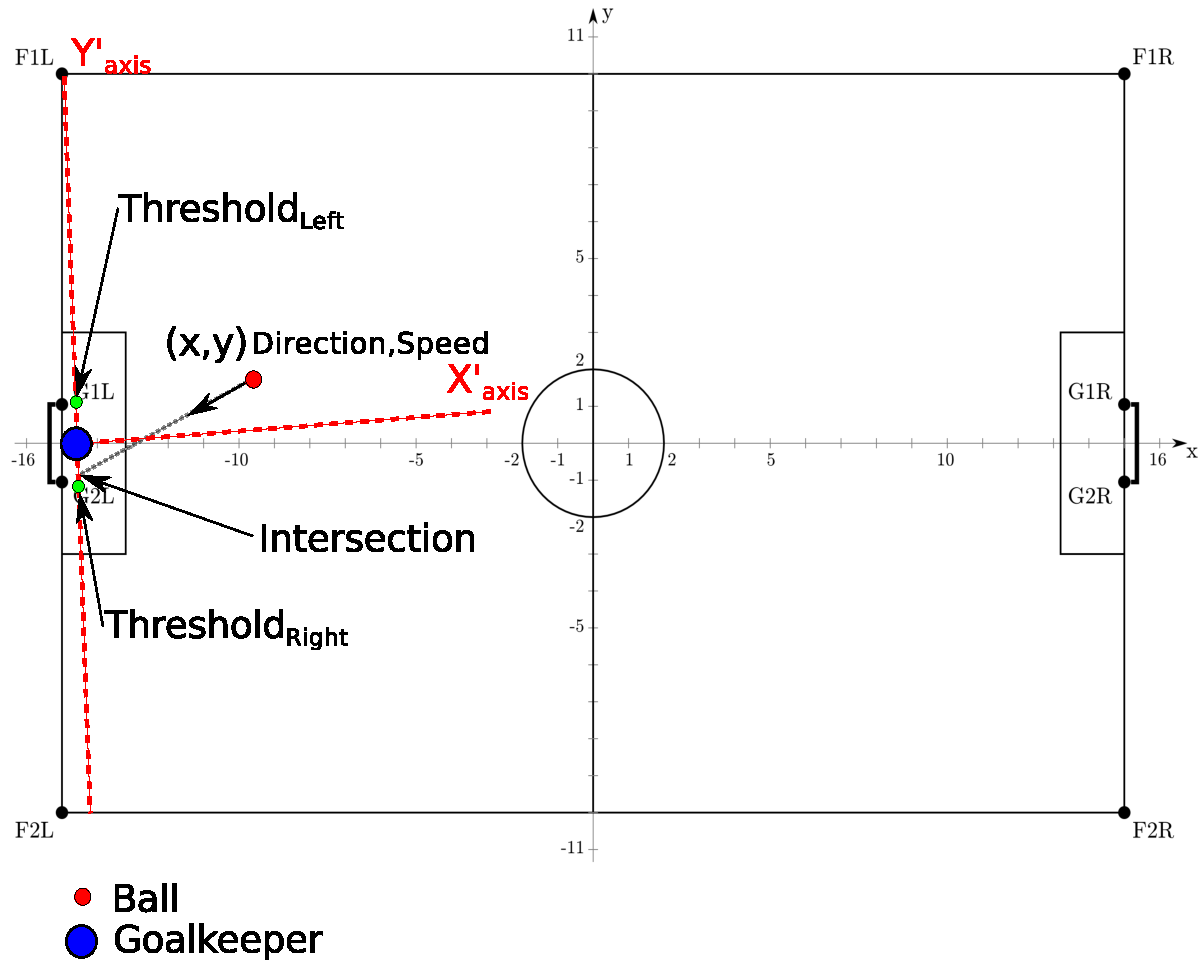
\includegraphics[trim = 0cm 11cm 0cm 0cm, clip,width=0.7\textwidth]{Chapter3/figures/Goalie.pdf}  
\end{figure} 
 	 
 	 
 	 \end{frame}  
 	 
 	 \begin{frame}
 	 \frametitle{Goalkeeper Fall Example}
 	 \begin{figure}[t!] 
	\centering
	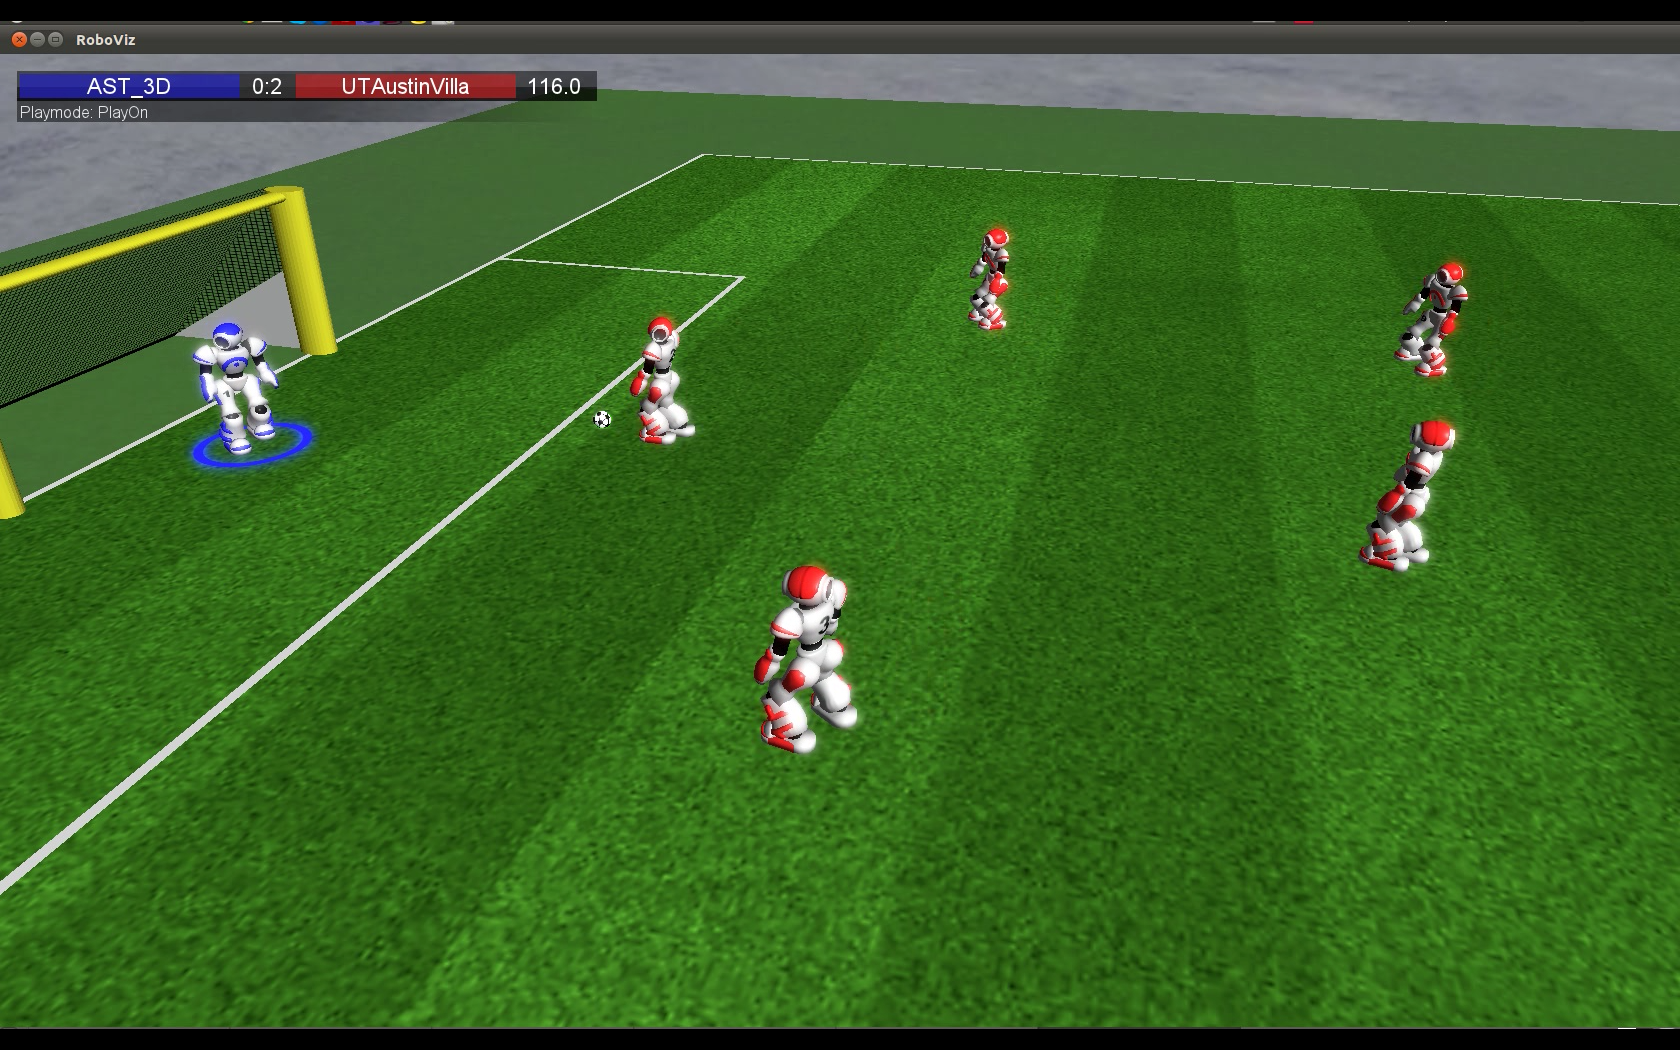
\includegraphics[trim = 5cm 10cm 30cm 5cm, clip,scale=0.15]{Chapter3/figures/GoalieFall.png}
	\quad 
	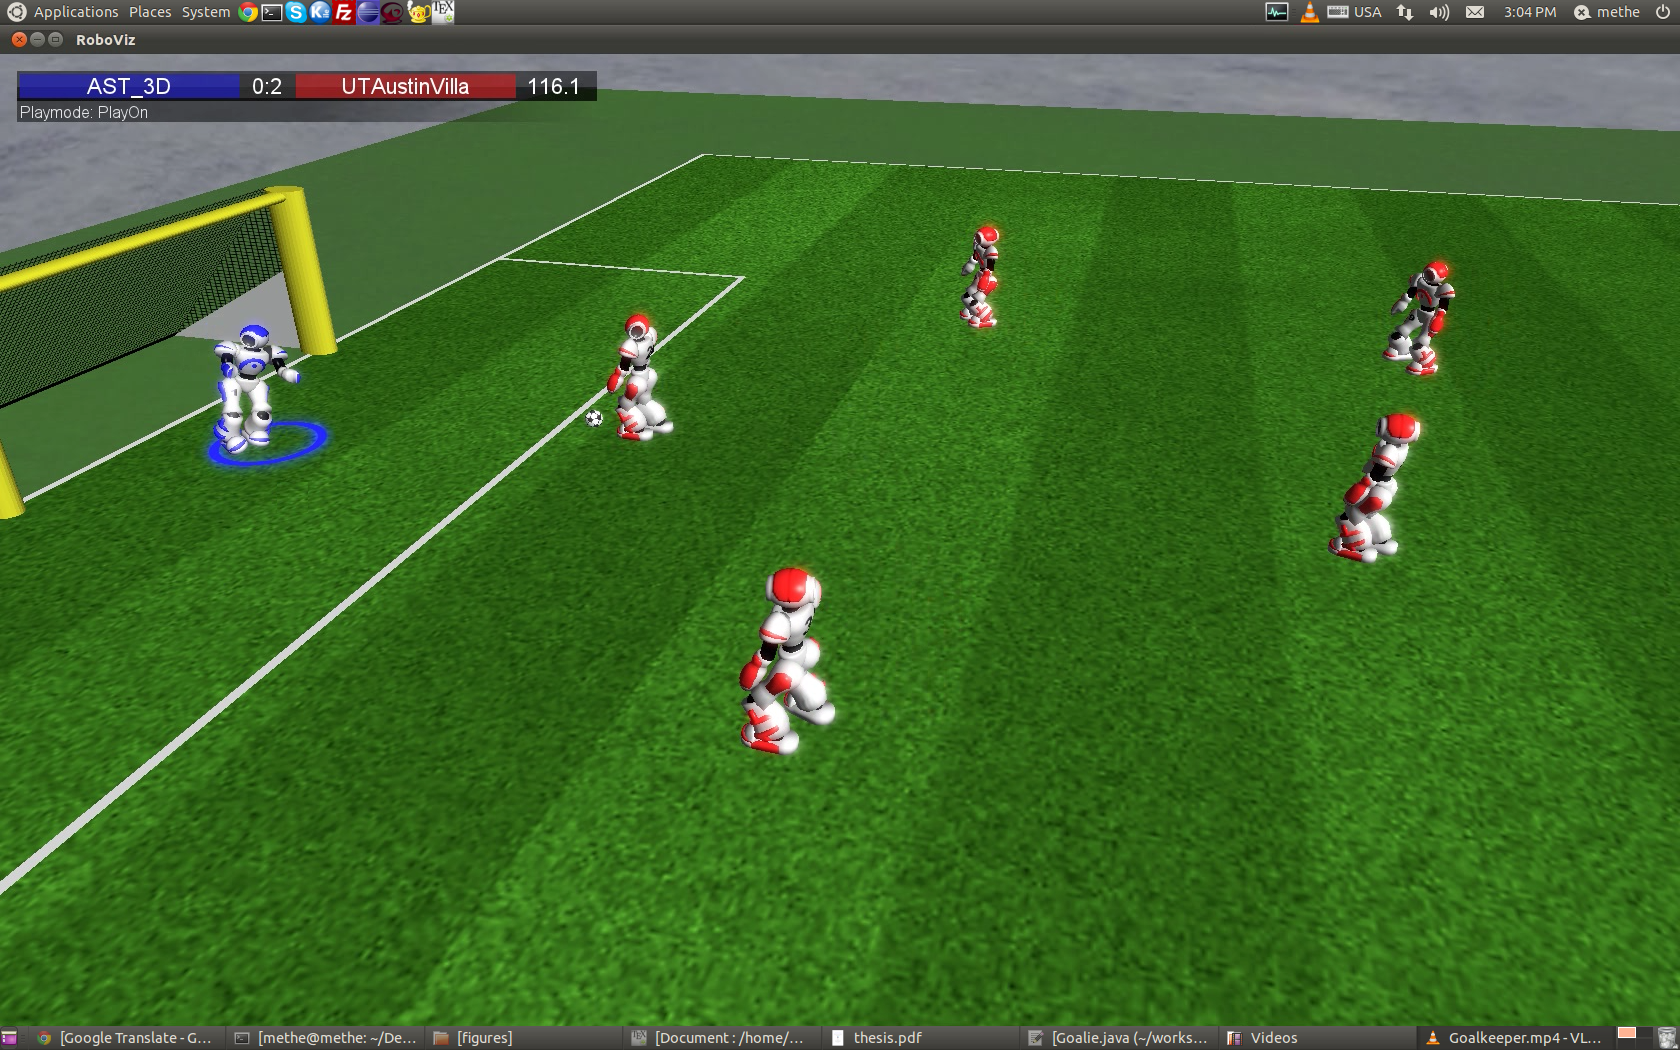
\includegraphics[trim = 5cm 10cm 30cm 5cm, clip,scale=0.15]{Chapter3/figures/GoalieFall2.png}\\
	\vspace*{0.2cm}
	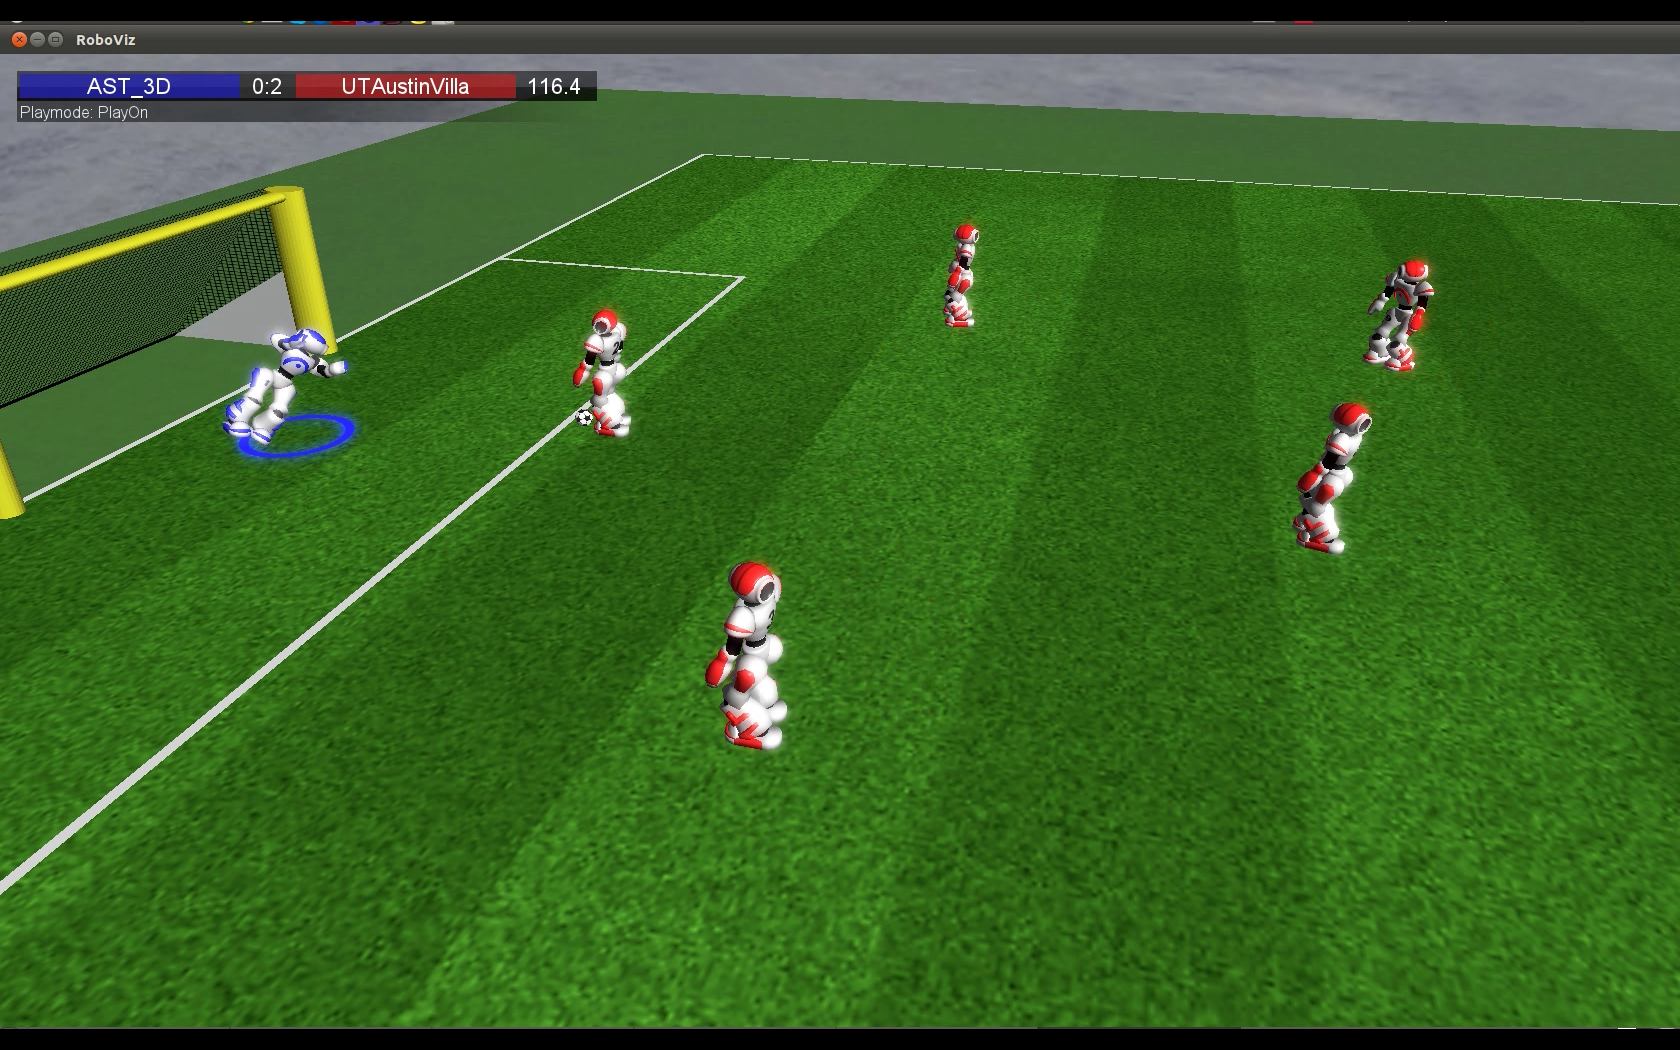
\includegraphics[trim = 5cm 10cm 30cm 5cm, clip,scale=0.15]{Chapter3/figures/GoalieFall3.png}
	\quad 
	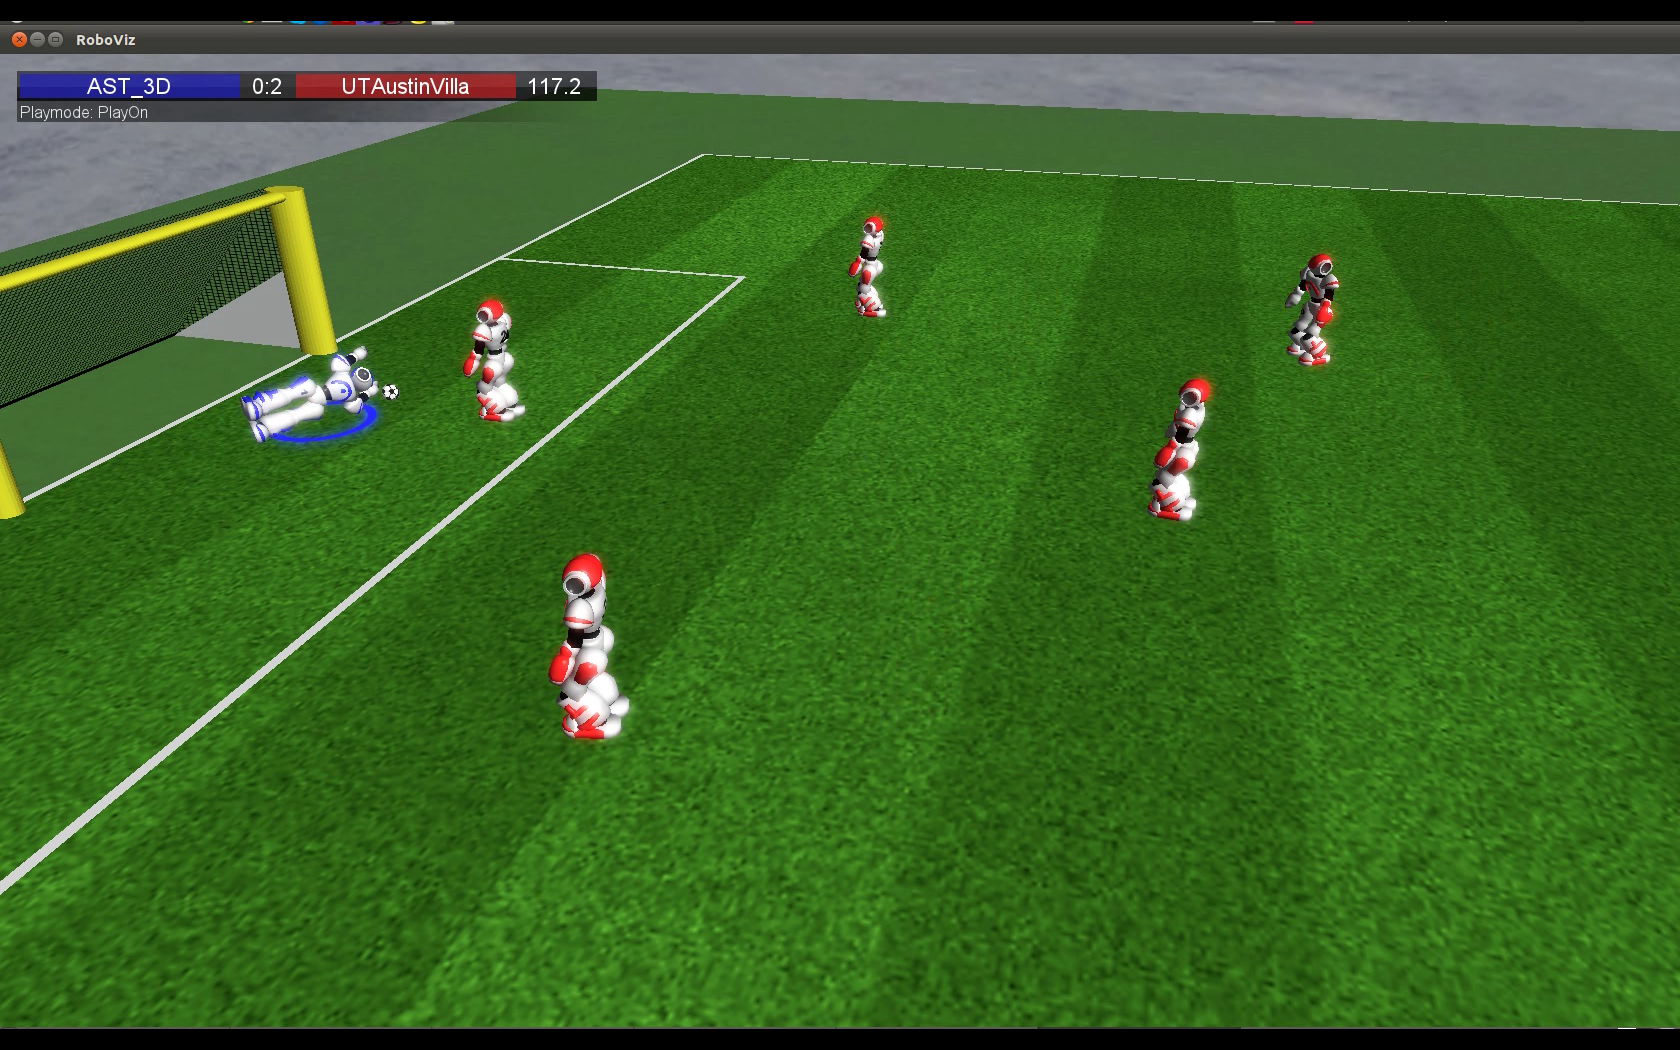
\includegraphics[trim = 5cm 10cm 30cm 5cm, clip,scale=0.15]{Chapter3/figures/GoalieFall4.png}
	\end{figure}
	\end{frame} 


  \section{Results}
  
  \subsection*{Motion}

  \frame
  {
    \frametitle{Motion Results and Improvements}
\begin{table}[t!]
\begin{center}
\begin{footnotesize}
\begin{tabular}{lrrrr}
\textbf{Motion Version} & \textbf{Walk(m/s)}	& \textbf{Turn(d/s)}	& \textbf{Kick(m)}&\textbf{Strong Kick(m)} \\
\midrule
Webots (Text-Based) 		& 0.11 				& 21 				& 3 				& - \\
FIIT (XML)				& 0.22 				& 25 				& 3 (4 Sec.) 		& 4 (5 Sec.) \\
\textbf{AST\_3D} 		& 0.45 	& 30 		& 3 (2.5 Sec.)& 5.5 (2.5 Sec.) \\
\end{tabular}
\end{footnotesize}
\end{center}
\end{table}

  }
  
  
  
  
  \subsection*{Communication Results}
  
  \frame
  {
    \frametitle{Communication Results}
	\begin{table}[b!]
	\begin{center}
	\begin{footnotesize}
    \begin{tabular}{lrr}
    \textbf{Communication Phase} 	& \textbf{Ideal (Cycles (Sec.))}			& \textbf{During Match (Cycles (Sec.))} \\
    \midrule
    Init Messages 					& 24  ( 0.48 ) 			& 24 	( 0.48 )		\\
    Coordination Messages			& 24  ( 0.48 )			& 42.5  ( 0.85 )		\\
    Action Messages 				    & 24  ( 0.48 )			& 24 ( 0.48 )	 		\\
    \end{tabular}
    \end{footnotesize}
\end{center}
\end{table}

  }


  \subsection*{Coordination}
  
  
  \frame
  {
    \frametitle{Coordination Beliefs (Global Ball Position)}
  \begin{figure}[h!]
\centering
  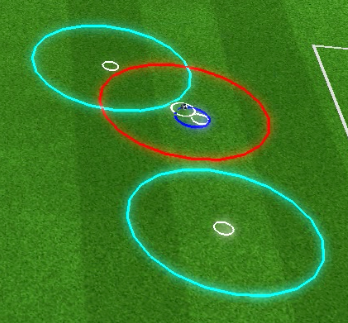
\includegraphics[height=3cm,width=3cm]{Chapter5/figures/BallObs1.png}\quad	
  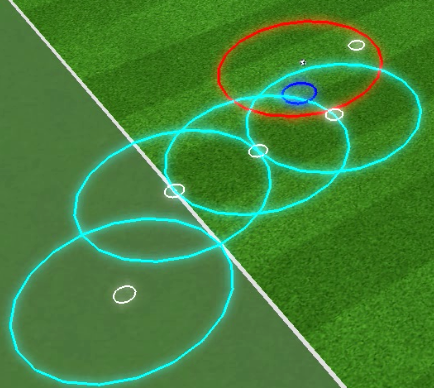
\includegraphics[height=3cm,width=3cm]{Chapter5/figures/BallObs2.png}\\ \vspace{0.2cm}
  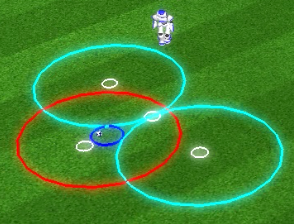
\includegraphics[height=3cm,width=3cm]{Chapter5/figures/BallObs3.png}\quad		
  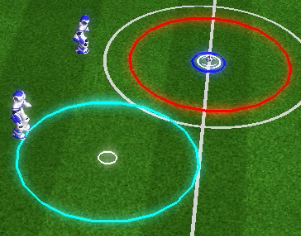
\includegraphics[height=3cm,width=3cm]{Chapter5/figures/BallObs4.png}
  
\end{figure}
  }
  
  
 \frame
  {
    \frametitle{Offensive Positioning 1}
    \begin{figure}[t!]
\centering
  \includegraphics[width=0.8\textwidth]{Chapter5/figures/3.pdf}
  
\end{figure}

 }
  
   \frame
  {
    \frametitle{Formation Consistency}
\begin{figure}[t!]
\centering
  \includegraphics[width=0.8\textwidth]{Chapter5/figures/4.pdf}
\end{figure}

  }  
 
  \frame
  {
    \frametitle{Defensive Positioning 1}
    \begin{figure}[t!]
\centering
  \includegraphics[width=0.8\textwidth]{Chapter5/figures/1.pdf}
\end{figure}

 }
 
 \frame
  {
    \frametitle{Defensive Positioning 2}
\begin{figure}[t!]
\centering
  \includegraphics[width=0.8\textwidth]{Chapter5/figures/2.pdf}
\end{figure}

  }
  
  
   \frame
  {
    \frametitle{Offensive Positioning 2}
\begin{figure}[t!]
\centering
  \includegraphics[width=0.8\textwidth]{Chapter5/figures/5.pdf}
\end{figure}

  }  

  \subsection*{GoalKeeper}
  \frame
  {
    \frametitle{Goalkeeper Results}
    
    \begin{table}[h!]
\begin{center}
    \begin{tabular}{lc}
    \textbf{GoalKeeper Type} 	& \textbf{Goals Conceded}\\
    \hline
    No Goalkeeper						& $\sim$ 7\\
    Goalkeeper with ``Empty'' Behavior	& $\sim$ 7\\
    Goalkeeper with ``Full'' Behavior	& $\sim$ 3\\
    \end{tabular}
\end{center}
\end{table}
    
    

  }
  
  \subsection*{Games}
  \frame
  {
    \frametitle{Full-Games Results}
    
\begin{table}[t!]
\begin{center}
    \begin{tabular}{cccccc}
    \textbf{Team} 	& \textbf{W} & \textbf{D} & \textbf{L} & \textbf{AGD} 	& \textbf{Games}   \\
    \midrule 
    MAK 		    & 2		& 0		& 0		& +2.0 		& 2 			\\
    L3M-SIM			& 3		& 2   	& 0		& +0.6 		& 5 			\\
    FARZANEGAN 		& 1		& 1		& 0		& +0.5 		& 2 			\\
    NomoFC 			& 1		& 2		& 0		& +0.3 		& 3 			\\
    Rail 			& 0		& 4		& 0		& 0.0 		& 4 			\\
    FUTK3D 			& 0		& 5		& 0		& 0.0 		& 5 			\\ 
    OxBlue 			& 0		& 0		& 2		& -1.5 		& 2 			\\
    BeeStanbul		& 0		& 0		& 3		& -4.0		& 3				\\
    UTAustinVilla 	& 0		& 0		& 4		& -5.2		& 4 			\\
    Robocanes 		& 0		& 0		& 1		& -6.0		& 1 			\\    
    \end{tabular}
\end{center}
\end{table}
  }


  \frame
  {
    \frametitle{Full-Games Results}
    
\begin{table}[t!]
\begin{center}
\begin{tabular}{l*{6}{c}r}
Team              	& P & W & D & L & F  & A & Pts \\ \hline
\textbf{AST3D} 		& \textbf{8} & \textbf{2} & \textbf{6} & \textbf{0} & \textbf{ 2} & \textbf{0} &  \textbf{12}  \\
NomoFC            	& 2 & 0 & 1 & 1 &  0 & 1 &  1  \\
L3M-SIM     		& 2 & 0 & 1 & 1 &  0 & 1 &  1  \\
Rail     		    & 2 & 0 & 2 & 0 &  0 & 0 &  2  \\
farzanegan     		& 2 & 0 & 2 & 0 &  0 & 0 &  2  \\
\end{tabular}
\end{center}
\end{table}
  }

  \section{Conclusion}

  \frame
  {
    \frametitle{Future Work} 
\begin{itemize}[<+->]
\item Probabilistic localization system
\item Dynamic Omni-Directional locomotiom
\item Passing
\item Participation in Robocup
\end{itemize}


  }

  \frame
  {
	\selectlanguage{greek}  
    \frametitle{\textit{Finally...}} 
    \begin{quote}
    \begin{LARGE}
    ��������� ����!
    \end{LARGE}
    \end{quote}
    \selectlanguage{english}

  }


\end{document}
